\newpage
\chapter*{Rozdział 3 \\ \vspace{1cm} Oszacowania modeli}
 \addcontentsline{toc}{chapter}{3. Oszacowania modeli}
 
W rozdziale tym przedstawione zostaną trzy modele ekonometryczne mogące służyć oszacowaniu czynników wpływających na prawdopodobieństwo zdobycia Oscara. Będą to: Liniowy Model Prawdopodobieństwa (LMP), Model Logit i Model Probit. Z modeli tych zostanie wybrany najlepszy, który potem posłuży do dalszych szczegółowych analiz.

\phantomsection				% do hiperlinków dla sekcji w spisie treści
\section*{3.1 Liniowy Model Prawdopodobieństwa}
\addcontentsline{toc}{section}{3.1 Liniowy Model Prawdopodobieństwa}

W tym podrozdziale oszacowany zostanie najprostszy do wyestymowania model z omawianych, czyli Liniowy Model Prawdopodobieństwa (LMP).

\vspace{0.5cm}

\textbf{Tabela 13. Ogólny model LMP}
\begin{stlog}	
. xi: reg oscar  budzet2000 i.gatunek ekranizacja roi przychody2000 kraj_prod nominacje zlote_globy bafta
 milosc czas_trwania
i.gatunek         _Igatunek_0-9       (naturally coded; _Igatunek_0 omitted)
{\smallskip}
      Source {\VBAR}       SS       df       MS              Number of obs =    1638
\HLI{13}{\PLUS}\HLI{30}           F( 19,  1618) =  126.33
       Model {\VBAR}  113.326224    19  5.96453809           Prob > F      =  0.0000
    Residual {\VBAR}  76.3935565  1618  .047214806           R-squared     =  0.5973
\HLI{13}{\PLUS}\HLI{30}           Adj R-squared =  0.5926
       Total {\VBAR}   189.71978  1637  .115894795           Root MSE      =  .21729
{\smallskip}
\HLI{15}{\TOPT}\HLI{63}{\DASH}
         oscar {\VBAR}      Coef.   Std. Err.      t    P>|t|     [95\% Conf. Interval]
\HLI{15}{\PLUS}\HLI{63}{\DASH}
    budzet2000 {\VBAR}  -7.00e-11   1.83e-10    -0.38   0.703    -4.30e-10    2.90e-10
   _Igatunek_1 {\VBAR}  -.0109619   .0164266    -0.67   0.505    -.0431815    .0212578
   _Igatunek_2 {\VBAR}   .0653794   .0302081     2.16   0.031     .0061283    .1246306
   _Igatunek_3 {\VBAR}   .0277427   .0301426     0.92   0.358    -.0313799    .0868654
   _Igatunek_4 {\VBAR}  -.0364617   .0286802    -1.27   0.204    -.0927159    .0197925
   _Igatunek_5 {\VBAR}   .0179434   .0240767     0.75   0.456    -.0292814    .0651683
   _Igatunek_6 {\VBAR}   .0440391   .0271553     1.62   0.105    -.0092242    .0973023
   _Igatunek_7 {\VBAR}   .0028486   .0241708     0.12   0.906    -.0445608    .0502579
   _Igatunek_8 {\VBAR}  -.0056704   .0255728    -0.22   0.825    -.0558297    .0444888
   _Igatunek_9 {\VBAR}  -.0388769   .0355595    -1.09   0.274    -.1086245    .0308706
   ekranizacja {\VBAR}  -.0099141   .0128952    -0.77   0.442    -.0352071     .015379
           roi {\VBAR}  -1.84e-08   1.62e-07    -0.11   0.910    -3.37e-07    3.00e-07
 przychody2000 {\VBAR}   4.56e-11   2.77e-11     1.65   0.100    -8.70e-12    9.99e-11
kraj_produkcji {\VBAR}  -.0277771   .0113187    -2.45   0.014    -.0499779   -.0055763
     nominacje {\VBAR}   .0812346    .003667    22.15   0.000     .0740421    .0884271
   zlote_globy {\VBAR}   .0745881   .0108014     6.91   0.000      .053402    .0957743
         bafta {\VBAR}   .0487341   .0086398     5.64   0.000     .0317878    .0656804
        milosc {\VBAR}   .0559628   .0201809     2.77   0.006     .0163793    .0955463
  czas_trwania {\VBAR}  -.0007682   .0003289    -2.34   0.020    -.0014133   -.0001231
         _cons {\VBAR}   .1058333   .0387433     2.73   0.006      .029841    .1818256
\HLI{15}{\BOTT}\HLI{63}{\DASH}

\end{stlog}

\textit{\footnotesize{Źródło: Opracowanie własne.}} \\	


W modelu ogólnym występuje kilka zmiennych nieistotnych na 5\%-owym poziomie istotności\footnote{Autor pracy założył poziom istotności dla wszystkich testów równy 5\%}, takich jak: budzet2000, _Igatunek_1, _Igatunek_3, _Igatunek_4, _Igatunek_5, _Igatunek_6, _Igatunek_7, _Igatunek_8, _Igatunek_9, ekranizacja, roi, przychody2000. W związku z tym postanowiono posłużyć się procedurą od ogólnego do szczegółowego, aby kolejno usuwając zmienne z modelu i badając ich łączną nieistotność (przy użyciu testu Walda) uzyskać model zagnieżdżony ze wszystkimi zmiennymi istotnymi na zadanym poziomie istotności. W tym miejscu zostanie pokazany tylko ostatni krok procedury, czyli sprawdzenie łącznej nieistotności wszystkich usuniętych w procedurze zmiennych i model finalny (tabela 14 i 15).

\vspace{0.5cm}

\textbf{Tabela 14. Test Walda dla wszystkich zmiennych usuwanych}
\begin{stlog}

. test _Igatunek_7 roi _Igatunek_8 budzet2000 _Igatunek_9 ekranizacja _Igatunek_1  _Igatunek_5 _Igatunek_3
 _Igatunek_4 przychody2000
{\smallskip}
 ( 1)  _Igatunek_7 = 0
 ( 2)  roi = 0
 ( 3)  _Igatunek_8 = 0
 ( 4)  budzet2000 = 0
 ( 5)  _Igatunek_9 = 0
 ( 6)  ekranizacja = 0
 ( 7)  _Igatunek_1 = 0
 ( 8)  _Igatunek_5 = 0
 ( 9)  _Igatunek_3 = 0
 (10)  _Igatunek_4 = 0
 (11)  przychody2000 = 0
       Constraint 11 dropped
{\smallskip}
       F( 10,  1618) =    0.67
            Prob > F =    0.7525

\end{stlog}

\textit{\footnotesize{Źródło: Opracowanie własne.}} \\	

Statystyka testu Walda na poziomie 0,67 i p-value tego testu równe 0,7525, czyli wskazują, iż nie ma podstaw do odrzucenia hipotezy zerowej o łącznej nieistotności zmiennych, czyli zmienne mogą zostać usunięte z modelu bez obaw o występowanie obciążenia Lovella.

 \vspace{0.5cm}

\textbf{Tabela 15. Zagnieżdżony model LMP}
\begin{stlog}	

. reg oscar _Igatunek_2 _Igatunek_6 kraj_prod nominacje zlote_globy bafta milosc czas_trwania
{\smallskip}
      Source {\VBAR}       SS       df       MS              Number of obs =    1663
\HLI{13}{\PLUS}\HLI{30}           F(  8,  1654) =  300.73
       Model {\VBAR}  113.994174     8  14.2492717           Prob > F      =  0.0000
    Residual {\VBAR}  78.3702278  1654  .047382242           R-squared     =  0.5926
\HLI{13}{\PLUS}\HLI{30}           Adj R-squared =  0.5906
       Total {\VBAR}  192.364402  1662  .115742721           Root MSE      =  .21767
{\smallskip}
\HLI{15}{\TOPT}\HLI{63}{\DASH}
         oscar {\VBAR}      Coef.   Std. Err.      t    P>|t|     [95\% Conf. Interval]
\HLI{15}{\PLUS}\HLI{63}{\DASH}
   _Igatunek_2 {\VBAR}   .0755959   .0252044     3.00   0.003       .02616    .1250318
   _Igatunek_6 {\VBAR}   .0504197   .0249408     2.02   0.043     .0015008    .0993386
kraj_produkcji {\VBAR}  -.0262216   .0110038    -2.38   0.017    -.0478044   -.0046388
     nominacje {\VBAR}   .0825513   .0034519    23.91   0.000     .0757806    .0893219
   zlote_globy {\VBAR}   .0748217   .0106572     7.02   0.000     .0539186    .0957248
         bafta {\VBAR}   .0490981    .008559     5.74   0.000     .0323105    .0658856
        milosc {\VBAR}   .0495576   .0198606     2.50   0.013     .0106031    .0885122
  czas_trwania {\VBAR}  -.0007373   .0002819    -2.62   0.009    -.0012903   -.0001844
         _cons {\VBAR}   .0990725    .032692     3.03   0.002     .0349504    .1631946
\HLI{15}{\BOTT}\HLI{63}{\DASH}

\end{stlog}

\textit{\footnotesize{Źródło: Opracowanie własne.}} \\

Statyka testu F równa 300,73 i p-value na poziomie 0.0000, czyli mniejsze od zakładanego 5\%-owego poziomu istotności sugerują, iż należy odrzucić hipotezę zerową o łącznej nieistotności zmienny objaśniających. Każda ze zmiennych objaśniających ma p-value mniejsze od 5\%, co oznacza, że zmienne są również osobno istotne (dla każdej z nich odrzucamy h0 o nieistotności). Model pod tym względem jest więc poprawnie zbudowany. Zmienności zmiennej zależnej jest wyjaśniane w 59,26\% przez zmienne niezależne.

Liniowy  model prawdopodobieństwa cechują jednak dwie poważne wady: nie ma gwarancji, że wartości dopasowane będą należeć do przedziału [0,1] oraz występuje w nim heteroskedastyczność, która przyczynia się niewłaściwego oszacowania błędów standardowych poszczególnych parametrów, co może wpłynąć na wnioski dotyczące istotności lub nieistotności zmiennych. Tabela 16 przedstawia test Breuscha-Pagana na heroskedastyczność reszt w modelu.
 
 \vspace{0.5cm}

\textbf{Tabela 16. Test Breuscha-Pagana na heroskedastyczność reszt}
\begin{stlog}	

. hettest,rhs 
{\smallskip}
Breusch-Pagan / Cook-Weisberg test for heteroskedasticity 
         Ho: Constant variance
         Variables: _Igatunek_2 _Igatunek_6 kraj_produkcji nominacje
                    zlote_globy bafta milosc czas_trwania
{\smallskip}
         chi2(8)      =   806.27
         Prob > chi2  =   0.0000

\end{stlog}

\textit{\footnotesize{Źródło: Opracowanie własne.}} \\	

Statystyka testowa równa 806,27 i p-value równe 0,0000 - mniejsze od zakładanego poziomu istotności, skłaniają do odrzucenia hipotezy zerowej o homoskedastyczności w modelu. Rozwiązaniem tego problemu może być oszacowanie modelu z użyciem błędów standardowych odpornych na heteroskedastyczność, czyli zastosowanie macierzy wariancji-kowariancji White'a (polecenie robust w programie Stata).

 \vspace{0.5cm}

\textbf{Tabela 17. Estymacja LMP  z zastosowaniem macierzy odpornej White'a}
\begin{stlog}	

. reg oscar _Igatunek_2 _Igatunek_6 kraj_prod nominacje zlote_globy bafta milosc czas_trwania, robust
{\smallskip}
Linear regression                                      Number of obs =    1663
                                                       F(  8,  1654) =  150.19
                                                       Prob > F      =  0.0000
                                                       R-squared     =  0.5926
                                                       Root MSE      =  .21767
{\smallskip}
\HLI{15}{\TOPT}\HLI{63}{\DASH}
               {\VBAR}               Robust
         oscar {\VBAR}      Coef.   Std. Err.      t    P>|t|     [95\% Conf. Interval]
\HLI{15}{\PLUS}\HLI{63}{\DASH}
   _Igatunek_2 {\VBAR}   .0755959   .0329737     2.29   0.022     .0109212    .1402705
   _Igatunek_6 {\VBAR}   .0504197   .0244259     2.06   0.039     .0025107    .0983287
kraj_produkcji {\VBAR}  -.0262216   .0111622    -2.35   0.019    -.0481151   -.0043282
     nominacje {\VBAR}   .0825513   .0057522    14.35   0.000     .0712689    .0938336
   zlote_globy {\VBAR}   .0748217   .0174394     4.29   0.000      .040616    .1090274
         bafta {\VBAR}   .0490981   .0149869     3.28   0.001     .0197028    .0784934
        milosc {\VBAR}   .0495576   .0239683     2.07   0.039     .0025462    .0965691
  czas_trwania {\VBAR}  -.0007373   .0002821    -2.61   0.009    -.0012906   -.0001841
         _cons {\VBAR}   .0990725   .0324942     3.05   0.002     .0353384    .1628066
\HLI{15}{\BOTT}\HLI{63}{\DASH}

\end{stlog}

\textit{\footnotesize{Źródło: Opracowanie własne.}} \\	

Ze względu na fakt, iż program Stata/IC 11 nie pozwala na zastosowanie komendy \textit{hettest,rhs} dla modelu z macierzą odporną White'a zastosowano inny równoważny test na heteroskedastyczność - test White'a (tabela 18).

 \vspace{0.5cm}

\textbf{Tabela 18. Test White'a na heteroskedastyczność reszt}
\begin{stlog}	

. whitetst
{\smallskip}
White's general test statistic :  449.6622  Chi-sq(38)  P-value =  8.3e-72

\end{stlog}

\textit{\footnotesize{Źródło: Opracowanie własne.}} \\	

Statystyka testu White'a równa 449,6622 i p-value równe 8.3e-72, czyli zdecydowanie mniejsze niż 5\% wskazują, iż problem heteroskedastyczność reszt dalej występuje, potwierdza to również przedstawiony poniżej rysunek 4. 


\begin{figure}[h]
\begin{centering}
  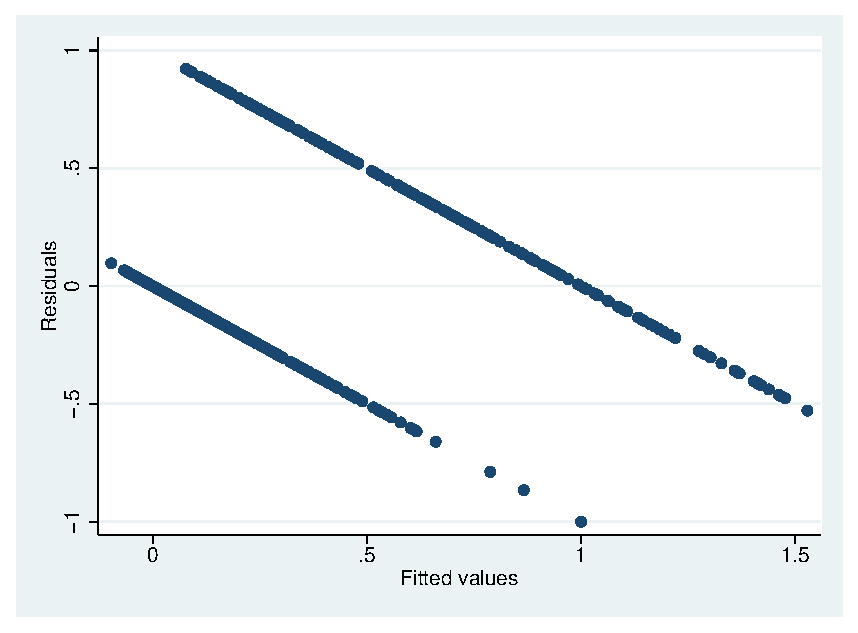
\includegraphics[height=3in]{Rysunki//resztyVSprzewidziane}
    \caption{\textbf{ Reszty vs. wartości przewidywane}}
\end{centering}
\end{figure}

\textit{\footnotesize{Źródło: Opracowanie własne.}} \\

Dla pełności analizy należy sprawdzić jeszcze czy wszystkie wartości dopasowane należą do przedziału [0,1], jeśli nie to jaki ich procent wykracza poza przedział. 

 \vspace{0.5cm}

\textbf{Tabela 19. Statystyki dotyczące wartości dopasowanych}
\begin{stlog}	

. predict xb1,xb
{\smallskip}
. sum xb1
{\smallskip}
    Variable {\VBAR}       Obs        Mean    Std. Dev.       Min        Max
\HLI{13}{\PLUS}\HLI{56}
         xb1 {\VBAR}      1663    .1334937    .2618942   -.096738   1.528635
{\smallskip}
. count if xb1<0 | xb1>1
  425

\end{stlog}

\textit{\footnotesize{Źródło: Opracowanie własne.}} \\	

Jak wynika z analizy tabeli 19 wartości dopasowane należą do przedziału od około -0.097 do 1,53, czyli znacząco wykraczają poza dopuszczalny przedział prawdopodobieństwa. Obserwacji wykraczających poza ten przedział jest dokładnie 425, czyli ponad jedna czwarta wszystkich.

Otrzymane wyniki testów na heteroskedastyczność reszt i zakres, w którym znajdują się wartości dopasowane, każą jednoznacznie wykluczyć Liniowy Model Prawdopodobieństwa jako narzędzie badania czynników wpływających na prawdopodobieństwo zdobycia Oscara.

\phantomsection				% do hiperlinków dla sekcji w spisie treści
\section*{3.2 Model Logit}
\addcontentsline{toc}{section}{3.2 Model Logit}

Kolejnym modelem omawianym w tym rozdziale pracy jest model Logit, różni się on od LMP dystrybuantą rozkładu prawdopodobieństwa. W LMP dystrybuanta miała postać funkcji liniowej, natomiast w modelu logitowym dystrybuantą jest dystrybunta rozkładu logistycznego o postaci: 
\begin{equation}
	\Lambda(x_i\beta)=\frac{e^{x_i\beta}}{1+e^{x_i\beta}}
\end{equation}
	
Podobnie jak w LMP analizę modelu logitowego należy zacząć od oszacowania modelu ogólnego, który przedstawia poniższa tabela:

\vspace{0.5cm}

\textbf{Tabela 20. Ogólny model logitowy}
\begin{stlog}	

. xi: logit oscar  budzet2000 i.gatunek ekranizacja roi przychody2000 kraj_prodnominacje zlote_globy 
bafta milosc czas_trwania
i.gatunek         _Igatunek_0-9       (naturally coded; _Igatunek_0 omitted)
{\smallskip}
Iteration 0:   log likelihood = -644.32291  
Iteration 1:   log likelihood = -281.35559  
Iteration 2:   log likelihood =  -239.5106  
Iteration 3:   log likelihood = -236.66683  
Iteration 4:   log likelihood =  -236.1946  
Iteration 5:   log likelihood = -235.78428  
Iteration 6:   log likelihood = -235.78225  
Iteration 7:   log likelihood = -235.78225  
{\smallskip}
Logistic regression                               Number of obs   =       1638
                                                  LR chi2(19)     =     817.08
                                                  Prob > chi2     =     0.0000
Log likelihood = -235.78225                       Pseudo R2       =     0.6341
{\smallskip}
\HLI{15}{\TOPT}\HLI{63}{\DASH}
         oscar {\VBAR}      Coef.   Std. Err.      z    P>|z|     [95\% Conf. Interval]
\HLI{15}{\PLUS}\HLI{63}{\DASH}
    budzet2000 {\VBAR}  -2.59e-09   4.68e-09    -0.55   0.580    -1.18e-08    6.57e-09
   _Igatunek_1 {\VBAR}  -.2373909   .4828453    -0.49   0.623     -1.18375    .7089686
   _Igatunek_2 {\VBAR}   .9471718   .6072435     1.56   0.119    -.2430034    2.137347
   _Igatunek_3 {\VBAR}   .8159699    .639625     1.28   0.202     -.437672    2.069612
   _Igatunek_4 {\VBAR}  -.5872744   .7910166    -0.74   0.458    -2.137639    .9630898
   _Igatunek_5 {\VBAR}   .4131266   .6023232     0.69   0.493    -.7674051    1.593658
   _Igatunek_6 {\VBAR}   .9000649   .5851035     1.54   0.124    -.2467169    2.046847
   _Igatunek_7 {\VBAR}   .0142123   .6206547     0.02   0.982    -1.202249    1.230673
   _Igatunek_8 {\VBAR}   .0969241   .8132038     0.12   0.905    -1.496926    1.690774
   _Igatunek_9 {\VBAR}  -.4927431   1.191666    -0.41   0.679    -2.828366     1.84288
   ekranizacja {\VBAR}  -.1438909   .2883711    -0.50   0.618    -.7090879    .4213061
           roi {\VBAR}  -.0001334   .0000993    -1.34   0.179     -.000328    .0000611
 przychody2000 {\VBAR}   2.11e-09   8.44e-10     2.50   0.012     4.58e-10    3.77e-09
kraj_produkcji {\VBAR}  -.7313622   .2766945    -2.64   0.008    -1.273674    -.189051
     nominacje {\VBAR}   .7179235   .0710326    10.11   0.000     .5787021    .8571449
   zlote_globy {\VBAR}   1.709133   .2826415     6.05   0.000     1.155166      2.2631
         bafta {\VBAR}   .7203465   .1709316     4.21   0.000     .3853267    1.055366
        milosc {\VBAR}   1.216106   .3967675     3.07   0.002     .4384561    1.993756
  czas_trwania {\VBAR}  -.0066497   .0080065    -0.83   0.406    -.0223422    .0090428
         _cons {\VBAR}  -3.372513    .958756    -3.52   0.000     -5.25164   -1.493386
\HLI{15}{\BOTT}\HLI{63}{\DASH}
Note: 2 failures and 0 successes completely determined.


\end{stlog}

\textit{\footnotesize{Źródło: Opracowanie własne.}} \\	

Jak można wywnioskować z tabeli 20, w modelu znajduje się kilka zmiennych nieistotnych na 5\%-owym poziomie istotności, są nimi: budzet2000, _Igatunek_1, _Igatunek_2, _Igatunek_3, _Igatunek_4, _Igatunek_5, _Igatunek_6, _Igatunek_7, _Igatunek_8, _Igatunek_9, ekranizacja, roi i czas trwania. W związku z tym zdecydowano się przeprowadzić podobnie jak w przypadku LMP procedurę od ogólnego do szczegółowego. Model zagnieżdżony otrzymany po przeprowadzeniu procedury został przedstawiony poniżej.

\vspace{0.5cm}

\textbf{Tabela 21. Zagnieżdżony model Logit i test Walda dla zmiennych usuniętych z modelu}

\begin{stlog}

. logit oscar _Igatunek_2 kraj_prod przychody2000 nominacje zlote_globy bafta milosc
{\smallskip}
Iteration 0:   log likelihood = -652.65521  
Iteration 1:   log likelihood =  -288.8549  
Iteration 2:   log likelihood = -247.94559  
Iteration 3:   log likelihood = -245.42423  
Iteration 4:   log likelihood = -245.41989  
Iteration 5:   log likelihood = -245.41989  
{\smallskip}
Logistic regression                               Number of obs   =       1657
                                                  LR chi2(7)      =     814.47
                                                  Prob > chi2     =     0.0000
Log likelihood = -245.41989                       Pseudo R2       =     0.6240
{\smallskip}
\HLI{15}{\TOPT}\HLI{63}{\DASH}
         oscar {\VBAR}      Coef.   Std. Err.      z    P>|z|     [95\% Conf. Interval]
\HLI{15}{\PLUS}\HLI{63}{\DASH}
   _Igatunek_2 {\VBAR}    1.09894   .4186544     2.62   0.009     .2783924    1.919488
kraj_produkcji {\VBAR}  -.7350574   .2651866    -2.77   0.006    -1.254814   -.2153012
 przychody2000 {\VBAR}   1.31e-09   4.83e-10     2.71   0.007     3.61e-10    2.26e-09
     nominacje {\VBAR}    .677297   .0601785    11.25   0.000     .5593492    .7952448
   zlote_globy {\VBAR}   1.642281   .2649008     6.20   0.000     1.123085    2.161477
         bafta {\VBAR}   .7662303    .168816     4.54   0.000      .435357    1.097104
        milosc {\VBAR}   1.040389   .3741386     2.78   0.005      .307091    1.773687
         _cons {\VBAR}   -4.07565   .2378775   -17.13   0.000    -4.541881   -3.609418
\HLI{15}{\BOTT}\HLI{63}{\DASH}
{\smallskip}
. test _Igatunek_7 _Igatunek_8 _Igatunek_9 _Igatunek_1 ekranizacja budzet2000 Igatunek_5 czas_trwania 
roi _Igatunek_5 _Igatunek_3 _Igatunek_6
{\smallskip}
 ( 1)  [oscar]_Igatunek_7 = 0
 ( 2)  [oscar]_Igatunek_8 = 0
 ( 3)  [oscar]_Igatunek_9 = 0
 ( 4)  [oscar]_Igatunek_1 = 0
 ( 5)  [oscar]ekranizacja = 0
 ( 6)  [oscar]budzet2000 = 0
 ( 7)  [oscar]_Igatunek_5 = 0
 ( 8)  [oscar]czas_trwania = 0
 ( 9)  [oscar]roi = 0
 (10)  [oscar]_Igatunek_5 = 0
 (11)  [oscar]_Igatunek_3 = 0
 (12)  [oscar]_Igatunek_6 = 0
       Constraint 10 dropped
{\smallskip}
           chi2( 11) =    8.74
         Prob > chi2 =    0.6455

\end{stlog}

\textit{\footnotesize{Źródło: Opracowanie własne.}} \\	

Statystyka testu ilorazu wiarygodności o wartości 814,47 i p-value równe 0,0000 każą odrzucić hipotezę zerową testu o łącznej nieistotności zmiennych. Wszystkie zmienne osobno również mają p-value mniejsze od 5\% co oznacza, że należy dla każdej z nich odrzucić hipotezę zerową o nieistotności. Statystyka testu Walda równa 8,74 i p-value wyraźnie większe od 5\% (0,6455 > 0,05) wskazują, iż nie ma podstaw do odrzucenia hipotezy zerowej o łącznej nieistotności zmiennych usuniętych z modelu.

Porównanie modelu ogólne i zagnieżdżonego na podstawie kryteriów informacyjnych BIC i AIC nie jest możliwe ze względu na różną liczbę obserwacji - model zagnieżdżony mający ich więcej niż ogólny byłby preferowany za względu na sposób wyliczania obu kryteriów (dzielenie przez N). Różnica w liczbie obserwacji bierze się z faktu, iż w modelu bez ograniczeń występuje zmienna budzet2000 dla której brakuje 19 obserwacji, a zmiennej tej nie ma w modelu z ograniczeniami.

\phantomsection				% do hiperlinków dla sekcji w spisie treści
\subsection*{3.2.1 Diagnostyka modelu Logit i testy jakości dopasowania}
\addcontentsline{toc}{subsection}{3.2.1 Diagnostyka modelu Logit i testy jakości dopasowania}
\vspace{0.5cm}

Przed przystąpieniem do interpretacji oszacowań modelu należy sprawdzić czy uzyskany model ma poprawną formę funkcyjną, czy jest dobrze dopasowany do danych. Do tego celu posłużą 3 testy diagnostyczne: linktest - test typu związku, test jakości dopasowania Perasona i test Hosmera-Lemeshow'a.


\vspace{0.5cm}

\textbf{Tabela 22. Test linktest dla modelu zagnieżdżonego}

\begin{stlog}
. linktest 
{\smallskip}
Iteration 0:   log likelihood = -652.65521  
Iteration 1:   log likelihood = -296.83394  
Iteration 2:   log likelihood = -279.56721  
Iteration 3:   log likelihood = -237.62155  
Iteration 4:   log likelihood = -235.86757  
Iteration 5:   log likelihood = -235.84334  
Iteration 6:   log likelihood = -235.84323  
Iteration 7:   log likelihood = -235.84323  
{\smallskip}
Logistic regression                               Number of obs   =       1657
                                                  LR chi2(2)      =     833.62
                                                  Prob > chi2     =     0.0000
Log likelihood = -235.84323                       Pseudo R2       =     0.6386
{\smallskip}
\HLI{13}{\TOPT}\HLI{64}
       oscar {\VBAR}      Coef.   Std. Err.      z    P>|z|     [95\% Conf. Interval]
\HLI{13}{\PLUS}\HLI{64}
        _hat {\VBAR}   .9408812    .055074    17.08   0.000     .8329381    1.048824
      _hatsq {\VBAR}  -.0504623   .0066712    -7.56   0.000    -.0635376    -.037387
       _cons {\VBAR}   .2421468   .1626919     1.49   0.137    -.0767234     .561017
\HLI{13}{\BOTT}\HLI{64}

\end{stlog}

\textit{\footnotesize{Źródło: Opracowanie własne.}} \\

Zarówno dla _hat, jak i _hatsq odrzucamy hipotezę zerową o nieistotności co oznacza, że dla wartości dopasowanych ważne są ich pierwsze i kolejne potęgi - forma funkcyjna jest niepoprawna.

\vspace{0.5cm}

\textbf{Tabela 23. Test Hosmera-Lemeshowa dla modelu zagnieżdżonego}

\begin{stlog}

. lfit, group(10) table
{\smallskip}
{\bftt{{\underbar{Logistic model for oscar, goodness-of-fit test}}}}
{\smallskip}
  (Table collapsed on quantiles of estimated probabilities)
  {\TLC}\HLI{7}{\TOPT}\HLI{8}{\TOPT}\HLI{7}{\TOPT}\HLI{7}{\TOPT}\HLI{7}{\TOPT}\HLI{7}{\TOPT}\HLI{7}{\TRC}
  {\VBAR} Group {\VBAR}   Prob {\VBAR} Obs_1 {\VBAR} Exp_1 {\VBAR} Obs_0 {\VBAR} Exp_0 {\VBAR} Total {\VBAR}
  {\LFTT}\HLI{7}{\PLUS}\HLI{8}{\PLUS}\HLI{7}{\PLUS}\HLI{7}{\PLUS}\HLI{7}{\PLUS}\HLI{7}{\PLUS}\HLI{7}{\RGTT}
  {\VBAR}     1 {\VBAR} 0.0086 {\VBAR}     0 {\VBAR}   1.4 {\VBAR}   167 {\VBAR} 165.6 {\VBAR}   167 {\VBAR}
  {\VBAR}     2 {\VBAR} 0.0094 {\VBAR}     0 {\VBAR}   1.5 {\VBAR}   165 {\VBAR} 163.5 {\VBAR}   165 {\VBAR}
  {\VBAR}     3 {\VBAR} 0.0115 {\VBAR}     0 {\VBAR}   1.7 {\VBAR}   166 {\VBAR} 164.3 {\VBAR}   166 {\VBAR}
  {\VBAR}     4 {\VBAR} 0.0171 {\VBAR}     0 {\VBAR}   2.6 {\VBAR}   165 {\VBAR} 162.4 {\VBAR}   165 {\VBAR}
  {\VBAR}     5 {\VBAR} 0.0184 {\VBAR}     1 {\VBAR}   2.9 {\VBAR}   165 {\VBAR} 163.1 {\VBAR}   166 {\VBAR}
  {\LFTT}\HLI{7}{\PLUS}\HLI{8}{\PLUS}\HLI{7}{\PLUS}\HLI{7}{\PLUS}\HLI{7}{\PLUS}\HLI{7}{\PLUS}\HLI{7}{\RGTT}
  {\VBAR}     6 {\VBAR} 0.0234 {\VBAR}     0 {\VBAR}   3.4 {\VBAR}   166 {\VBAR} 162.6 {\VBAR}   166 {\VBAR}
  {\VBAR}     7 {\VBAR} 0.0374 {\VBAR}     6 {\VBAR}   4.9 {\VBAR}   159 {\VBAR} 160.1 {\VBAR}   165 {\VBAR}
  {\VBAR}     8 {\VBAR} 0.0854 {\VBAR}    13 {\VBAR}   9.5 {\VBAR}   153 {\VBAR} 156.5 {\VBAR}   166 {\VBAR}
  {\VBAR}     9 {\VBAR} 0.5610 {\VBAR}    55 {\VBAR}  41.7 {\VBAR}   111 {\VBAR} 124.3 {\VBAR}   166 {\VBAR}
  {\VBAR}    10 {\VBAR} 1.0000 {\VBAR}   147 {\VBAR} 152.4 {\VBAR}    18 {\VBAR}  12.6 {\VBAR}   165 {\VBAR}
  {\BLC}\HLI{7}{\BOTT}\HLI{8}{\BOTT}\HLI{7}{\BOTT}\HLI{7}{\BOTT}\HLI{7}{\BOTT}\HLI{7}{\BOTT}\HLI{7}{\BRC}
{\smallskip}
       number of observations =      1657
             number of groups =        10
      Hosmer-Lemeshow chi2(8) =        21.72
                  Prob > chi2 =         0.0055
                 
\end{stlog}

\textit{\footnotesize{Źródło: Opracowanie własne.}} \\

Statystyka testu Pearsona wynosi 1981,2, a p-value 0.0000 < 0,05 co oznacza, że należy odrzucić hipotezę zerową wskazującą na poprawność formy funkcyjnej. Również test Hosmera-Lemeshowa wskazuje na niepoprawną formę funkcyjną - statystyka testowa=21,72 i p-value=0,0055 (mniejsze od 5\%), skłaniają do odrzucenia hipotezy zerowej o poprawnej postaci funkcyjnej modelu.

\vspace{0.5cm}

\textbf{Tabela 24. Test Pearsona dla modelu zagnieżdżonego}

\begin{stlog}

. estat gof 
{\smallskip}
{\bftt{{\underbar{Logistic model for oscar, goodness-of-fit test}}}}
{\smallskip}
       number of observations =      1657
 number of covariate patterns =      1654
           Pearson chi2(1646) =      1981.20
                  Prob > chi2 =         0.0000

\end{stlog}

\textit{\footnotesize{Źródło: Opracowanie własne.}} \\


W tej sytuacji gdy wszystkie testy wskazują na niepoprawność formy funkcyjnej modelu należy zastanowić się nad poszukaniem dodatkowych istotnych zmiennych objaśniających, które można by dodać do modelu, lub nad wprowadzeniem interakcji pomiędzy zmiennymi niezależnymi. W przypadku tego modelu oba sposoby zawiodły - nie udało się odnaleźć dodatkowych istotnych zmiennych ani interakcji. W takich sytuacjach jak sugerują autorzy książki \textit{Logistic Regression with Stata} \cite{chen10} można się posłużyć modelem Boxa-Tidwella (komenda \textit{boxtid} w programie Stata )\footnote{ Przykład zastosowania modelu Boxa-Tidwella do transformacji zmiennej niezależnej w modelu Logit można odnaleźć w trzecim rozdziale (\textit{Logistic Regression Diagnostics}) wyżej wspomnianej książki}. Model ten transformuje zmienną niezależną używając transformacji potęgowej i znajduje najlepszą jej potęgę na podstawie oszacowania największej wiarygodności (odpowiednik transformacji Boxa-Coxa). Transformacja zmiennej objaśniającej $x$ jest dokonywana według wzoru:


\begin{equation}
	\beta_0+\beta_1x^p
\end{equation}
\vspace{0.4cm}

Oszacowana potęga $p$ (na wydruku ze Staty pod nazwą $p1$) przyjmuje wartości ze zbioru liczb rzeczywistych, aby ułatwić późniejszą interpretację przetransformowanych zmiennych przyjęło się przybliżać $p$ do jednej z liczb ze zbioru $ P = \{-2,-1,-0.5,0,0.5,1,2\}$. W przypadku, gdy oszacowane $p$ jest bliskie zera to zmienną niezależną $x$ transformuje się używając logarytmu naturalnego do postaci $ln(x)$, w pozostałych przypadkach zmienną niezależną podnosi się do najbliższej potęgi ze zbioru $P$.\footnote{ Szczegółowy opis działania komendy \textit{boxtid} i samego modelu Boxa-Tidewella został zawarty w artykule P. Roystona i G. Ambler \textit{Nonlinear regression models involving power or exponential functions of covariates} opublikowanym w 1999 roku w \textit{Stata Technical Bulletin 49 \cite{royston99}}.} W tabeli 25 zaprezentowane jest wydruk testu transformacji zmiennych niezależnych przy użyciu komendy \textit{boxtid}. Opcja zero() w tym teście została użyta ze względu na przeważającą liczbę obserwacji zerowych dla zmiennych nominacje, zlote_globy i bafta. Opcja ta zapewnia nie uwzględnianie obserwacji zerowych przy dopasowywaniu modelu z potęgami - pod uwagę brane są tylko obserwacje mogące wpływać na nieliniowość zmiennej objaśniającej.

\vspace{1.5cm}
\textbf{Tabela 25. Test transformacji zmiennych dla modelu zagnieżdżonego Logit}
\begin{stlog}
. boxtid logit oscar _Igatunek_2 kraj_prod przychody2000 nominacje zlote_globy bafta milosc, 
zero(nominacje zlote_globy bafta) 
Iteration 0:  Deviance =  427.4704
(unprofitable step attempted, step length divided by 10)
Iteration 1:  Deviance =  410.3915 (change = -17.07888)
Iteration 2:  Deviance =  410.3759 (change = -.0156017)
Iteration 3:  Deviance =  410.3746 (change = -.0012795)
Iteration 4:  Deviance =  410.3745 (change =  -.000127)
-> gen double Iprzy__1 = X{\caret}0.5491-.3674405338 if e(sample) 
-> gen double Iprzy__2 = X{\caret}0.5491*ln(X)+.6700151336 if e(sample) 
   (where: X = przychody2000/1000000000)
-> gen double Inomi__1 = X{\caret}0.1671-.8424693853 if e(sample) 
-> gen double Inomi__2 = X{\caret}0.1671*ln(X)+.8642909775 if e(sample) 
   (where: X = nominacje/10)
-> gen double Izlot__1 = zlote_globy{\caret}0.2492-1.161232965 if e(sample) 
-> gen double Izlot__2 = zlote_globy{\caret}0.2492*ln(zlote_globy)-.6965615002 if e(sa
> mple) 
-> gen double Ibaft__1 = bafta{\caret}0.2163-1.167894033 if e(sample) 
-> gen double Ibaft__2 = bafta{\caret}0.2163*ln(bafta)-.8380787452 if e(sample) 
[Total iterations: 16]
Box-Tidwell regression model

Logistic regression                               Number of obs   =       1657
                                                  LR chi2(11)     =     894.94
                                                  Prob > chi2     =     0.0000
Log likelihood = -205.18721                       Pseudo R2       =     0.6856
{\smallskip}
\HLI{13}{\TOPT}\HLI{64}
       oscar {\VBAR}      Coef.   Std. Err.      z    P>|z|     [95\% Conf. Interval]
\HLI{13}{\PLUS}\HLI{64}
    Iprzy__1 {\VBAR}   1.029977   .6067958     1.70   0.090    -.1593207    2.219275
    Iprzy_p1 {\VBAR}   .0053793   .5716119     0.01   0.992    -1.114959    1.125718
    Inomi__1 {\VBAR}   9.716826   2.955026     3.29   0.001     3.925082    15.50857
    Inomi_p1 {\VBAR}  -.0017302   .6638651    -0.00   0.998    -1.302882    1.299421
    Izlot__1 {\VBAR}   1.809972   .3147959     5.75   0.000     1.192983    2.426961
    Izlot_p1 {\VBAR}   .0003923   .5272507     0.00   0.999       -1.033    1.033785
    Ibaft__1 {\VBAR}   1.265426   .3160349     4.00   0.000     .6460094    1.884843
    Ibaft_p1 {\VBAR}    .000038   .3781499     0.00   1.000    -.7411223    .7411983
 _Igatunek_2 {\VBAR}   .6675307   .4445605     1.50   0.133    -.2037919    1.538853
kraj_produ{\tytilde}i {\VBAR}  -.6652295   .2711986    -2.45   0.014    -1.196769     -.13369
      milosc {\VBAR}   1.119758    .413176     2.71   0.007     .3099482    1.929568
       _cons {\VBAR}   2.689804    .428151     6.28   0.000     1.850643    3.528964
\HLI{13}{\BOTT}\HLI{64}
przychody2000| 7.37e-10   4.24e-10      1.739 Nonlin. dev. 0.922   (P = 0.337)
      p1 |   .5490613   .5305962      1.035
------------------------------------------------------------------------------
nominacje|      .6618   .0606394     10.914   Nonlin. dev. 56.291  (P = 0.000)
      p1 |   .1670898   .0681398      2.452
------------------------------------------------------------------------------
zlote_globy| 1.284998   .2322075      5.534   Nonlin. dev. 5.699   (P = 0.017)
      p1 |   .2492006   .2913101      0.855
------------------------------------------------------------------------------
bafta    |   .6230049   .1535889      4.056   Nonlin. dev. 6.261   (P = 0.012)
      p1 |   .2162805   .2988773      0.724
------------------------------------------------------------------------------
Deviance:  410.375.
\end{stlog}
\textit{\footnotesize{Źródło: Opracowanie własne.}} \\

Dla trzech zmiennych p-value testu na nieliniowość ma wartość mniejszą od 5\%, co oznacza konieczność odrzucenia hipotezy  zerowej o liniowości tych zmiennych, są nimi: nominacje (P = 0,000), zlote_globy (P = 0,017) i bafta (P = 0,012). Dla zmiennej przychody2000 p-value równe 0,337 wskazuje na brak podstaw do odrzucenia h0 o liniowej formie zmiennej. Dla wszystkich trzech zmiennych $p1$ jest bliższe 0 niż 0,5, dla zmiennej nominacje jest to około 0,167, dla zmiennej zlote_globy 0,2492, a dla zmiennej bafta 0,2163. W tej sytuacji należy przetransformować wszystkie trzy zmienne przy użyciu logarytmu naturalnego. Taka postać transformacji jest prawdopodobnie spowodowana spadającym krańcowym wpływem danej zmiennej objaśniającej na objaśnianą. Czyli z każdą kolejną nominacją/nagrodą wpływ na prawdopodobieństwo zdobycia Oscara jest mniejszy. W związku z wynikami testu sprawdzającego nieliniowość zmiennych niezależnych oszacowano nowy model logitowy ze zmiennymi ln_nom, ln_zg i ln_baf będącymi logarytmami naturalnymi zmiennych: nominacje, zlote_globy i bafta.

\vspace{0.5cm}
\textbf{Tabela 26. Model Logit po transformacji}
\begin{stlog}
. logit oscar _Igatunek_2 kraj_prod przychody2000 ln_nom ln_zg ln_baf milosc
Iteration 0:   log likelihood = -652.65521  
Iteration 1:   log likelihood = -343.52428  
Iteration 2:   log likelihood = -293.05786  
Iteration 3:   log likelihood = -286.11262  
Iteration 4:   log likelihood = -286.07875  
Iteration 5:   log likelihood = -286.07874  

Logistic regression                               Number of obs   =       1657
                                                  LR chi2(7)      =     733.15
                                                  Prob > chi2     =     0.0000
Log likelihood = -286.07874                       Pseudo R2       =     0.5617
\HLI{15}{\TOPT}\HLI{63}{\DASH}
         oscar {\VBAR}      Coef.   Std. Err.      z    P>|z|     [95\% Conf. Interval]
\HLI{15}{\PLUS}\HLI{63}{\DASH}
   _Igatunek_2 {\VBAR}   1.298812   .4099903     3.17   0.002      .495246    2.102379
kraj_produkcji {\VBAR}  -.6795015   .2417108    -2.81   0.005    -1.153246    -.205757
 przychody2000 {\VBAR}   9.58e-10   4.65e-10     2.06   0.039     4.73e-11    1.87e-09
        ln_nom {\VBAR}    2.43787   .1658775    14.70   0.000     2.112757    2.762984
         ln_zg {\VBAR}    1.91387   .7098043     2.70   0.007     .5226786     3.30506
        ln_baf {\VBAR}   1.620144   .4197213     3.86   0.000     .7975055    2.442783
        milosc {\VBAR}   1.076732   .3544051     3.04   0.002     .3821111    1.771354
         _cons {\VBAR}  -3.707948   .2136529   -17.36   0.000      -4.1267   -3.289196
\HLI{15}{\BOTT}\HLI{63}{\DASH}
 \end{stlog}
\textit{\footnotesize{Źródło: Opracowanie własne.}} \\

Wszystkie zmienne w modelu są łącznie istotne (LR chi2(7)=733,15, p-value=0,0000 < 0,05) i każda zmienna z osobna ma p-value mniejsze od 5\% co wskazuje na konieczność odrzucenia hipotezy zerowej o nieistotności poszczególnych zmiennych. Psudo R$^{2}$ wskazuje, iż zmienność została wyjaśniona  w około 56,15\%. Przeprowadzenie ponownych testów poprawności funkcyjnej modelu pozwoli odpowiedzieć na pytanie czy transformacja zmiennych przyniosła pożądany skutek.

\vspace{0.5cm}

\textbf{Tabela 27. Linktest dla modelu z transformacjami}
\begin{stlog}
. linktest
Iteration 0:   log likelihood = -652.65521  
Iteration 1:   log likelihood = -340.18544  
Iteration 2:   log likelihood = -300.42787  
Iteration 3:   log likelihood = -290.19594  
Iteration 4:   log likelihood = -289.39801  
Iteration 5:   log likelihood = -289.36772  
Iteration 6:   log likelihood = -289.36772  

Logistic regression                               Number of obs   =       1657
                                                  LR chi2(2)      =     726.57
                                                  Prob > chi2     =     0.0000
Log likelihood = -289.36772                       Pseudo R2       =     0.5566

\HLI{13}{\TOPT}\HLI{64}
       oscar {\VBAR}      Coef.   Std. Err.      z    P>|z|     [95\% Conf. Interval]
\HLI{13}{\PLUS}\HLI{64}
        _hat {\VBAR}   .9450873    .071231    13.27   0.000     .8054771    1.084698
      _hatsq {\VBAR}  -.0251742   .0231046    -1.09   0.276    -.0704584      .02011
       _cons {\VBAR}   .0769665   .1584652     0.49   0.627    -.2336197    .3875527
\HLI{13}{\BOTT}\HLI{64}
 \end{stlog}
\textit{\footnotesize{Źródło: Opracowanie własne.}} \\

Tym razem zmienna \textit{_hat} okazała się istotna (p-value = 0 - należy odrzucić h0 o nieistotności zmiennej na każdym poziomie istotności), a w przypadku zmiennej \textit{_hatsq} niema podstaw do odrzucenia h0 o nieistotności (p.value = 0,276 > 0,05). Model z trzema zmiennymi w logarytmach ma poprawną formę funkcyjną. 

\vspace{0.5cm}
\textbf{Tabela 28. Test Pearsona i test Hosmera-Lemeshowa dla modelu z transformacjami}
\begin{stlog}
. estat gof
{\bftt{{\underbar{Logistic model for oscar, goodness-of-fit test}}}}
{\smallskip}
       number of observations =      1657
 number of covariate patterns =      1654
           Pearson chi2(1646) =      1440.50
                  Prob > chi2 =         0.9999
{\smallskip}
. lfit, group(10) table
{\smallskip}
{\bftt{{\underbar{Logistic model for oscar, goodness-of-fit test}}}}
{\smallskip}
  (Table collapsed on quantiles of estimated probabilities)
  {\TLC}\HLI{7}{\TOPT}\HLI{8}{\TOPT}\HLI{7}{\TOPT}\HLI{7}{\TOPT}\HLI{7}{\TOPT}\HLI{7}{\TOPT}\HLI{7}{\TRC}
  {\VBAR} Group {\VBAR}   Prob {\VBAR} Obs_1 {\VBAR} Exp_1 {\VBAR} Obs_0 {\VBAR} Exp_0 {\VBAR} Total {\VBAR}
  {\LFTT}\HLI{7}{\PLUS}\HLI{8}{\PLUS}\HLI{7}{\PLUS}\HLI{7}{\PLUS}\HLI{7}{\PLUS}\HLI{7}{\PLUS}\HLI{7}{\RGTT}
  {\VBAR}     1 {\VBAR} 0.0142 {\VBAR}     1 {\VBAR}   2.3 {\VBAR}   165 {\VBAR} 163.7 {\VBAR}   166 {\VBAR}
  {\VBAR}     2 {\VBAR} 0.0151 {\VBAR}     1 {\VBAR}   2.4 {\VBAR}   165 {\VBAR} 163.6 {\VBAR}   166 {\VBAR}
  {\VBAR}     3 {\VBAR} 0.0170 {\VBAR}     2 {\VBAR}   2.6 {\VBAR}   164 {\VBAR} 163.4 {\VBAR}   166 {\VBAR}
  {\VBAR}     4 {\VBAR} 0.0235 {\VBAR}     4 {\VBAR}   3.3 {\VBAR}   161 {\VBAR} 161.7 {\VBAR}   165 {\VBAR}
  {\VBAR}     5 {\VBAR} 0.0244 {\VBAR}     4 {\VBAR}   4.0 {\VBAR}   162 {\VBAR} 162.0 {\VBAR}   166 {\VBAR}
  {\LFTT}\HLI{7}{\PLUS}\HLI{8}{\PLUS}\HLI{7}{\PLUS}\HLI{7}{\PLUS}\HLI{7}{\PLUS}\HLI{7}{\PLUS}\HLI{7}{\RGTT}
  {\VBAR}     6 {\VBAR} 0.0261 {\VBAR}     5 {\VBAR}   4.2 {\VBAR}   161 {\VBAR} 161.8 {\VBAR}   166 {\VBAR}
  {\VBAR}     7 {\VBAR} 0.0408 {\VBAR}     3 {\VBAR}   4.9 {\VBAR}   162 {\VBAR} 160.1 {\VBAR}   165 {\VBAR}
  {\VBAR}     8 {\VBAR} 0.0799 {\VBAR}    10 {\VBAR}   9.8 {\VBAR}   156 {\VBAR} 156.2 {\VBAR}   166 {\VBAR}
  {\VBAR}     9 {\VBAR} 0.5908 {\VBAR}    49 {\VBAR}  45.4 {\VBAR}   117 {\VBAR} 120.6 {\VBAR}   166 {\VBAR}
  {\VBAR}    10 {\VBAR} 0.9999 {\VBAR}   143 {\VBAR} 143.1 {\VBAR}    22 {\VBAR}  21.9 {\VBAR}   165 {\VBAR}
  {\BLC}\HLI{7}{\BOTT}\HLI{8}{\BOTT}\HLI{7}{\BOTT}\HLI{7}{\BOTT}\HLI{7}{\BOTT}\HLI{7}{\BOTT}\HLI{7}{\BRC}
{\smallskip}
       number of observations =      1657
             number of groups =        10
      Hosmer-Lemeshow chi2(8) =         3.23
                  Prob > chi2 =         0.9194
\end{stlog}
\textit{\footnotesize{Źródło: Opracowanie własne.}} \\

\vspace{0.5cm}
\textbf{Tabela 29. Porównanie modeli przed i po transformacji trzech zmiennych niezależnych}
\begin{stlog}
. fitstat, using(m2) 
Measures of Fit for logit of oscar
{\smallskip}
                               Current             Saved        Difference
Model:                           logit             logit
N:                                1657              1657                 0
Log-Lik Intercept Only        -652.655          -652.655             0.000
Log-Lik Full Model            -286.079          -245.420           -40.659
D                              572.157(1649)     490.840(1649)      81.318(0)
LR                             733.153(7)        814.471(7)         81.318(0)
Prob > LR                        0.000             0.000                 .
McFadden's R2                    0.562             0.624            -0.062
McFadden's Adj R2                0.549             0.612            -0.062
ML (Cox-Snell) R2                0.358             0.388            -0.031
Cragg-Uhler(Nagelkerke) R2       0.656             0.712            -0.056
McKelvey \& Zavoina's R2          0.610             0.751            -0.142
Efron's R2                       0.590             0.635            -0.044
Tjur's Discrimination Coef       0.596             0.650            -0.053
Variance of y*                   8.425            13.221            -4.796
Variance of error                3.290             3.290             0.000
Count R2                         0.937             0.941            -0.004
Adj Count R2                     0.532             0.559            -0.027
AIC                            588.157           506.840            81.318
AIC/N                            0.355             0.306             0.049
BIC                            631.460           550.142            81.318
{\smallskip}
Difference of   81.318 in BIC provides very strong support for saved model.
{\smallskip}
Note: p-value for difference in LR is only valid if models are nested.
\end{stlog}
\textit{\footnotesize{Źródło: Opracowanie własne.}} \\

Podobnie jak linktest tak i dwa kolejne testy sprawdzające dopasowanie modelu do danych wskazały, iż nowy model ma prawidłową formę funkcyjną.  Statystyka testu Pearsona wyniosła 1440,50, a p-value 0,9999, co wskazuje na przyjęcie hipotezy zerowej mówiącej o poprawności zastosowanej formy funkcyjnej. Podobnie statystyka testu  Hosmera-Lemeshowa równa 3,23 i p-value równe 0,9194 (>0,05) wskazują na brak podstaw do odrzucenia h0 mówiącej o prawidłowości formy funkcyjnej. W tym miejscu należałoby porównać model przed transformacją i po transformacji zmiennych, aby zobaczyć jak zlogarytmowanie wpłynęło na najważniejsze miary dopasowania modelu.

Tabel 29 przedstawia porównanie modeli przed i po transformacji trzech zmiennych niezależnych. \textit{Current logit} oznacza model po transformacjach, a \textit{Saved logit} oznacza model przed transformacjami. Niemal wszystkie współczynniki determinacji modelu wskazują, iż model ze zmiennymi niezlogarytmowanymi lepiej reprezentował dane, lepiej przewidywał sukcesy i porażki, miał niższe kryteria informacyjne. Mimo to należy posłużyć się modelem gorzej dopasowanym , ale z poprawną formą funkcyjną. Tak więc model po transformacjach dla zmiennej ukrytej y$_{i}^{*}$ byłby wyjaśniany w 61\%, gdyby zmienna ta była bezpośrednio obserwowalna (McKelvey-Zavoina R2). Przewiduje on trafnie sukcesy i porażki w 93,7\% na co wskazuje liczebnościowe R$^{2}$. Skorygowane liczebnościowe R$^{2}$ (Adj Count R2) pokazuje natomiast, że dzięki zmiennym objaśniającym model trafnie przewiduje sukcesy i porażki w 53,2\%.

\begin{figure}[h]
\begin{centering}
  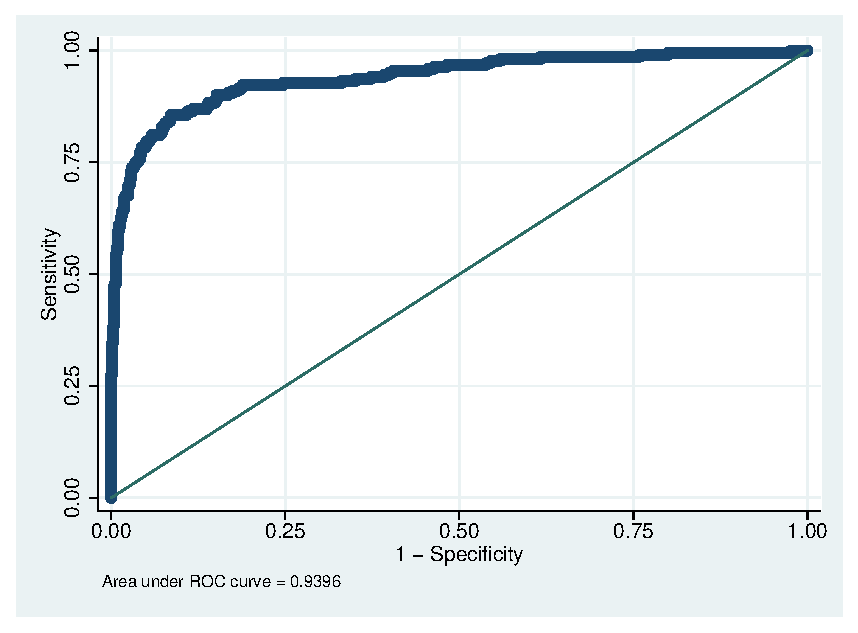
\includegraphics[height=3in]{Rysunki//ROC2}
    \caption{\textbf{Krzywa ROC}}
\end{centering}
\end{figure}
\textit{\footnotesize{Źródło: Opracowanie własne.}} \\

\vspace{0.5cm}
\textbf{Tabela 30. Pole pod krzywą ROC }
\begin{stlog}
. lroc
{\smallskip}
Logistic model for oscar
{\smallskip}
number of observations =     1657
area under ROC curve   =   0.9396 
 \end{stlog}
\textit{\footnotesize{Źródło: Opracowanie własne.}} \\

Pole pod krzywą ROC jest to procent dobrze zakwalifikowanych pozytywnych i negatywnych odpowiedzi przy różnych wyborach punktu rozdzielającego decyzję. Im bliższa jedynce wartość pola tym model jest lepiej dopasowany do danych wejściowych. Tabela 30 wskazuje na bardzo dobre dopasowanie modelu - pole pod krzywą ROC wynosi 0,9396.

\vspace{0.5cm}
\begin{figure}[h]
\begin{centering}
  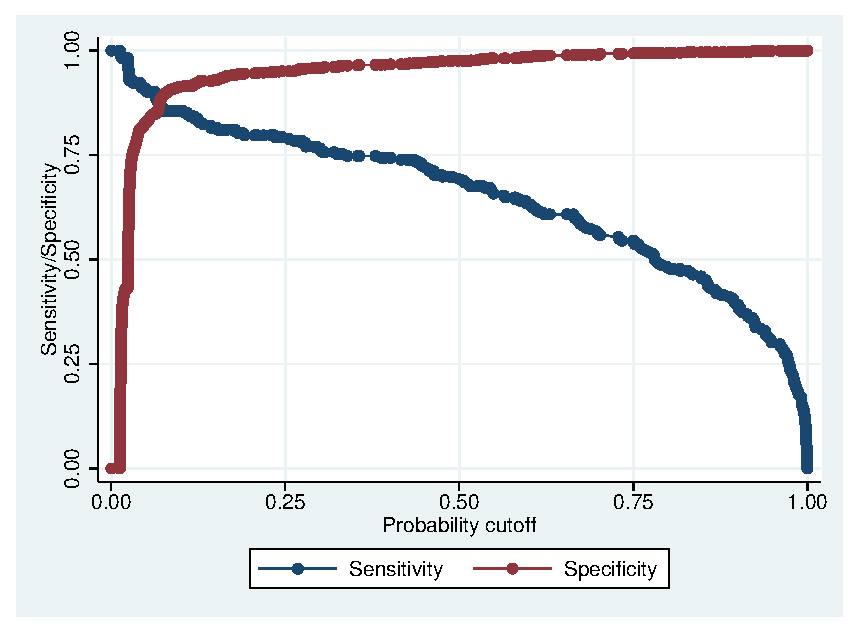
\includegraphics[height=3in]{Rysunki//SENS2}
    \caption{\textbf{Wrażliwość i Specyficzność}}
\end{centering}
\end{figure}
\textit{\footnotesize{Źródło: Opracowanie własne.}} \\

Wykres wrażliwości i specyficzności wskazuje prawdopodobieństwo ucięcia, czyli poziom rozgraniczenia maksymalizującego trafność klasyfikacji wartości dopasowanych. Z rysunku 6 wynika, iż najlepsze ucięcie powinno mieć miejsce w punkcie 0,05. Dla tego punktu wyznaczona została tablica klasyfikacji.

\vspace{0.5cm}
\textbf{Tabela 31. Tablica klasyfikacji dla punktu odcięcia równego 0,05 }
\begin{stlog}
. lstat,cutoff(0.05)
{\smallskip}
Logistic model for oscar
{\smallskip}
              \HLI{8} True \HLI{8}
Classified {\VBAR}         D            {\tytilde}D  {\VBAR}      Total
\HLI{11}{\PLUS}\HLI{26}{\PLUS}\HLI{11}
     +     {\VBAR}       201           248  {\VBAR}        449
     -     {\VBAR}        21          1187  {\VBAR}       1208
\HLI{11}{\PLUS}\HLI{26}{\PLUS}\HLI{11}
   Total   {\VBAR}       222          1435  {\VBAR}       1657
\vspace{0.3cm}
Classified + if predicted Pr(D) >= .05
True D defined as oscar != 0
\HLI{50}
Sensitivity                     Pr( +| D)   90.54\%
Specificity                     Pr( -|{\tytilde}D)   82.72\%
Positive predictive value       Pr( D| +)   44.77\%
Negative predictive value       Pr({\tytilde}D| -)   98.26\%
\HLI{50}
False + rate for true {\tytilde}D        Pr( +|{\tytilde}D)   17.28\%
False - rate for true D         Pr( -| D)    9.46\%
False + rate for classified +   Pr({\tytilde}D| +)   55.23\%
False - rate for classified -   Pr( D| -)    1.74\%
\HLI{50}
Correctly classified                        83.77\%
\HLI{50}
 \end{stlog}
\textit{\footnotesize{Źródło: Opracowanie własne.}} \\

Tabela 31 wskazuje iż na 222 filmy, które zdobyły Oscara, model prawidłowo przewidział aż 201 z nich, czyli blisko 91\% (wrażliwość), a jedynie 21 zostało błędnie zakwalifikowanych (9\%). Natomiast spośród 1435 filmów, które nie otrzymały żadnej statuetki, model prawidłowo przewidział 1187, czyli około 83\% (specyficzność), błędnie zakwalifikowanych obserwacji było w tej kategorii około 17\%. Łącznie 83,77\% wszystkich obserwacji zostało trafnie zakwalifikowanych, co wydaje się bardzo dobrym wynikiem. 

\vspace{0.5cm}
\textbf{Tabela 32. Test Współliniowości zmiennych }
\begin{stlog}
. collin _Igatunek_2 kraj_prod przychody2000 ln_nom ln_zg ln_baf milosc
(obs=1657)
{\smallskip}
  Collinearity Diagnostics
{\smallskip}
                        SQRT                   R-
  Variable      VIF     VIF    Tolerance    Squared
----------------------------------------------------
_Igatunek_2      1.05    1.02    0.9531      0.0469
kraj_produkcji      1.03    1.02    0.9678      0.0322
przychody2000      1.17    1.08    0.8528      0.1472
    ln_nom      1.83    1.35    0.5470      0.4530
     ln_zg      1.52    1.23    0.6579      0.3421
    ln_baf      1.56    1.25    0.6404      0.3596
    milosc      1.01    1.00    0.9923      0.0077
----------------------------------------------------
  Mean VIF      1.31
{\smallskip}
                           Cond
        Eigenval          Index
---------------------------------
    1     3.1127          1.0000
    2     1.5024          1.4394
    3     0.9743          1.7874
    4     0.8126          1.9572
    5     0.5384          2.4044
    6     0.4980          2.5001
    7     0.3291          3.0754
    8     0.2324          3.6594
---------------------------------
 Condition Number         3.6594 
 Eigenvalues \& Cond Index computed from scaled raw sscp (w/ intercept)
 Det(correlation matrix)    0.3797
\end{stlog}

\textit{\footnotesize{Źródło: Opracowanie własne.}} \\

Ostatnim koniecznym testem jest test na występowanie współliniowości zmiennych objaśniających w modelu. Współliniowość zmiennych ma miejsce gdy jedną zmienną można uzyskać jako kombinację liniową pozostałych. Występowanie współliniowości może stanowić obciążenie dla oszacowanego ilorazu szans, gdyż powoduje ono znaczący wzrost błędów standardowych w modelu. Aby sprawdzić czy zjawisko współliniowości zmiennych objaśniających występuje w oszacowanym modelu logitowym posłużono się komendą \textit{collin} w programie Stata. Tabela 32 przedstawia wyniki tego testu. Niska wartość statystyk \textit{VIF}, \textit{Condition Number} i \textit{Condition Index} (poniżej 10) wskazuje na brak współliniowości pomiędzy zmiennymi niezależnymi i ich stabilność.

\phantomsection				% do hiperlinków dla sekcji w spisie treści
\section*{3.3 Model Probit}
\addcontentsline{toc}{section}{3.3 Model Probit}

Model probitowy podobnie jak model logitowy jest modelem dedykowanym binarnej zmiennej zależnej. Główna różnica pomiędzy Logitem, a Probitem polega na postaci dystrybuanty rozkładu prawdopodobieństwa - dla modelu logitowego jest to dystrybuanta rozkładu logitowego $\Lambda(x_i\beta)$, a dla modelu probitowego jest nią dystrybuanta standaryzowanego rozkładu normalnego $\Phi(x_i\beta)$. Podobnie jak w przypadku modeli Logit i LMP na początku wyestymowano ogólny model Probit (tabela 33).

\vspace{2cm}
\textbf{Tabela 33. Model Probit ogólny}
\begin{stlog}
. xi: probit oscar  budzet2000 i.gatunek ekranizacja roi przychody2000 kraj_prod nominacje zlote_globy bafta
 milosc czas_trwania
i.gatunek         _Igatunek_0-9       (naturally coded; _Igatunek_0 omitted)
{\smallskip}
Iteration 0:   log likelihood = -644.32291  
Iteration 1:   log likelihood = -252.37591  
Iteration 2:   log likelihood = -233.42969  
Iteration 3:   log likelihood = -233.07162  
Iteration 4:   log likelihood = -232.57344  
Iteration 5:   log likelihood = -232.57049  
Iteration 6:   log likelihood = -232.57049  
{\smallskip}
Probit regression                                 Number of obs   =       1638
                                                  LR chi2(18)     =     823.50
                                                  Prob > chi2     =     0.0000
Log likelihood = -232.57049                       Pseudo R2       =     0.6390
{\smallskip}
\HLI{15}{\TOPT}\HLI{63}{\DASH}
         oscar {\VBAR}      Coef.   Std. Err.      z    P>|z|     [95\% Conf. Interval]
\HLI{15}{\PLUS}\HLI{63}{\DASH}
    budzet2000 {\VBAR}  -2.05e-09   2.36e-09    -0.87   0.386    -6.67e-09    2.58e-09
   _Igatunek_1 {\VBAR}  -.1380634   .2283552    -0.60   0.545    -.5856314    .3095046
   _Igatunek_2 {\VBAR}   .4729934   .3124234     1.51   0.130    -.1393452    1.085332
   _Igatunek_3 {\VBAR}   .3290652    .334237     0.98   0.325    -.3260273    .9841578
   _Igatunek_4 {\VBAR}  -.2879733   .3982407    -0.72   0.470    -1.068511    .4925641
   _Igatunek_5 {\VBAR}   .1873941   .2964899     0.63   0.527    -.3937154    .7685035
   _Igatunek_6 {\VBAR}   .3683275   .2977027     1.24   0.216     -.215159     .951814
   _Igatunek_7 {\VBAR}  -.0186585   .3088218    -0.06   0.952    -.6239381    .5866212
   _Igatunek_8 {\VBAR}  -.0237881   .3833369    -0.06   0.951    -.7751147    .7275385
   _Igatunek_9 {\VBAR}  -.2951531    .613072    -0.48   0.630    -1.496752    .9064459
   ekranizacja {\VBAR}  -.0461109   .1434598    -0.32   0.748     -.327287    .2350652
           roi {\VBAR}  -.0000491   .0000469    -1.05   0.295     -.000141    .0000428
 przychody2000 {\VBAR}   1.03e-09   4.26e-10     2.43   0.015     1.98e-10    1.87e-09
kraj_produkcji {\VBAR}  -.3755098   .1370391    -2.74   0.006    -.6441015    -.106918
     nominacje {\VBAR}   .3835013   .0353914    10.84   0.000     .3141353    .4528672
   zlote_globy {\VBAR}   .8039639   .1324897     6.07   0.000     .5442889    1.063639
         bafta {\VBAR}    .375868   .0860155     4.37   0.000     .2072806    .5444554
        milosc {\VBAR}   .5883756   .2029476     2.90   0.004     .1906055    .9861456
  czas_trwania {\VBAR}  -.0036616   .0039782    -0.92   0.357    -.0114588    .0041355
         _cons {\VBAR}  -1.769618   .4736227    -3.74   0.000    -2.697901   -.8413347
\HLI{15}{\BOTT}\HLI{63}{\DASH}
Note: 2 failures and 15 successes completely determined.
\end{stlog}
\textit{\footnotesize{Źródło: Opracowanie własne.}} \\

Na 5\%-owym poziomie istotności nie ma podstaw do odrzucenia hipotezy zerowej o nieistotności dla następujących zmiennych: budzet2000, _Igatunek_1, _Igatunek_2, _Igatunek_3, _Igatunek_4, _Igatunek_5, _Igatunek_6, _Igatunek_7, _Igatunek_8, _Igatunek_9, ekranizacja, roi, czas_trwania. W celu pozbycia się zmiennych nieistotnych z modelu zastosowano procedurę od ogólnego do szczegółowego, po przeprowadzeniu której uzyskano model ze wszystkimi zmiennymi istotnymi. W tym miejscu zostanie zaprezentowany tylko ostatni etap procedury.

\vspace{0.5cm}
\textbf{Tabela 34. Test Walda dla zmiennych usuniętych z modelu}
\begin{stlog}
. test _Igatunek_7 _Igatunek_8 ekranizacja _Igatunek_9 _Igatunek_1 _Igatunek_4  czas_trwania roi 
budzet2000 _Igatunek_3 _Igatunek_5 _Igatunek_6
{\smallskip}
 ( 1)  [oscar]_Igatunek_7 = 0
 ( 2)  [oscar]_Igatunek_8 = 0
 ( 3)  [oscar]ekranizacja = 0
 ( 4)  [oscar]_Igatunek_9 = 0
 ( 5)  [oscar]_Igatunek_1 = 0
 ( 6)  [oscar]_Igatunek_4 = 0
 ( 7)  [oscar]czas_trwania = 0
 ( 8)  [oscar]roi = 0
 ( 9)  [oscar]budzet2000 = 0
 (10)  [oscar]_Igatunek_3 = 0
 (11)  [oscar]_Igatunek_5 = 0
 (12)  [oscar]_Igatunek_6 = 0
{\smallskip}
           chi2( 12) =    8.11
         Prob > chi2 =    0.7761
\end{stlog}
\textit{\footnotesize{Źródło: Opracowanie własne.}} \\

Statystyka testu Walda (8,11) i p-value(0,7761 < 0,05) wskazują, iż nie ma podstaw do odrzucenia h0 o łącznej nieistotności zmiennych usuniętych z modelu.

\vspace{0.5cm}
\textbf{Tabela 35. Model Probit zagnieżdżony}
\begin{stlog}
. probit oscar _Igatunek_2 kraj_prod przychody2000 nominacje zlote_globy bafta milosc
{\smallskip}
Iteration 0:   log likelihood = -652.65521  
Iteration 1:   log likelihood = -260.18232  
Iteration 2:   log likelihood = -241.49363  
Iteration 3:   log likelihood = -241.25808  
Iteration 4:   log likelihood = -241.25791  
Iteration 5:   log likelihood = -241.25791  
{\smallskip}
Probit regression                                 Number of obs   =       1657
                                                  LR chi2(6)      =     822.79
                                                  Prob > chi2     =     0.0000
Log likelihood = -241.25791                       Pseudo R2       =     0.6303
{\smallskip}
\HLI{15}{\TOPT}\HLI{63}{\DASH}
         oscar {\VBAR}      Coef.   Std. Err.      z    P>|z|     [95\% Conf. Interval]
\HLI{15}{\PLUS}\HLI{63}{\DASH}
   _Igatunek_2 {\VBAR}   .5389003   .2270996     2.37   0.018     .0937931    .9840074
kraj_produkcji {\VBAR}  -.3809342   .1314571    -2.90   0.004    -.6385853   -.1232831
 przychody2000 {\VBAR}   6.53e-10   2.34e-10     2.79   0.005     1.94e-10    1.11e-09
     nominacje {\VBAR}   .3678263   .0306592    12.00   0.000     .3077353    .4279173
   zlote_globy {\VBAR}   .7954267   .1267459     6.28   0.000     .5470092    1.043844
         bafta {\VBAR}   .3983077   .0842226     4.73   0.000     .2332344    .5633811
        milosc {\VBAR}   .5150889    .194828     2.64   0.008     .1332331    .8969446
         _cons {\VBAR}  -2.212964   .1096436   -20.18   0.000    -2.427861   -1.998066
\HLI{15}{\BOTT}\HLI{63}{\DASH}
Note: 0 failures and 15 successes completely determined.
\end{stlog}
\textit{\footnotesize{Źródło: Opracowanie własne.}} \\

Statystyka LR chi2(6) = 822,79 i p-value=0,0000 < 0,05 wskazuje na konieczność odrzucenia hipotezy zerowej o łącznej nieistotności wszystkich zmiennych. Również p-value każdej zmiennej z osobna jest mniejsze od 5\% co każe odrzucić h0 dla każdej zmiennej o nieistotności - wszystkie zmienne są osobno istotne. Model wyjaśnia około 63,03\% zmienności (Pseudo R$^{2}$). 

Podobnie jak w przypadku modelu Logit nie możemy porównywać modeli ogólnego i zagnieżdżonego na podstawie kryteriów informacyjnych BIC i AIC ze względu na różnicę w liczbie obserwacji w obu modelach - wynika ona z braku 19 obserwacji zmiennej budzet2000.

\phantomsection				% do hiperlinków dla sekcji w spisie treści
\subsection*{3.3.1 Diagnostyka modelu Probit i testy jakości dopasowania}
\addcontentsline{toc}{subsection}{3.3.1 Diagnostyka modelu Probit i testy jakości dopasowania}
\vspace{0.5cm}

Aby móc interpretować oszacowania modelu należy najpierw sprawdzić czy model zagnieżdżony ma poprawną formę funkcyjną, czy jest dobrze dopasowany. W tym celu wykorzystane zostaną trzy testy diagnostyczne: test typu związku (linktest), test jakości dopasowania (goodness of fit) i test Hosmera-Lemeshow'a.

\vspace{0.5cm}
\textbf{Tabela 36. Test linktest dla zagnieżdżonego modelu Probit}
\begin{stlog}
. linktest
{\smallskip}
Iteration 0:   log likelihood = -652.65521  
Iteration 1:   log likelihood = -244.58488  
Iteration 2:   log likelihood = -230.27775  
Iteration 3:   log likelihood =  -230.1471  
Iteration 4:   log likelihood = -230.14708  
Iteration 5:   log likelihood = -230.14708  
{\smallskip}
Probit regression                                 Number of obs   =       1657
                                                  LR chi2(2)      =     845.02
                                                  Prob > chi2     =     0.0000
Log likelihood = -230.14708                       Pseudo R2       =     0.6474
{\smallskip}
\vspace{0.5cm}
\HLI{13}{\TOPT}\HLI{64}
       oscar {\VBAR}      Coef.   Std. Err.      z    P>|z|     [95\% Conf. Interval]
\HLI{13}{\PLUS}\HLI{64}
        _hat {\VBAR}   .9539365    .049118    19.42   0.000      .857667    1.050206
      _hatsq {\VBAR}  -.0997172    .013172    -7.57   0.000     -.125534   -.0739005
       _cons {\VBAR}   .1917916    .090433     2.12   0.034     .0145461     .369037
\HLI{13}{\BOTT}\HLI{64}
\end{stlog}
\textit{\footnotesize{Źródło: Opracowanie własne.}} \\

Test typu związku wskazuje, iż dla zmiennej \textit{_hat} należy odrzucić hipotezę zerową o nieistotności (p-value=0,000 < 0,05), podobnie dla \textit{_hatsq} odrzucamy hipotezę o nieistotności (p-value=0,0000 < 0,05), co oznacza, że dla wartości dopasowanych istotne są również dalsze potęgi. 

\vspace{0.5cm}
\textbf{Tabela 37. Test jakości dopasowania dla zagnieżdżonego modelu Probit}
\begin{stlog}
. estat gof
{\smallskip}
{\bftt{{\underbar{Probit model for oscar, goodness-of-fit test}}}}
{\smallskip}
       number of observations =      1657
 number of covariate patterns =      1654
           Pearson chi2(1646) =      6344.33
                  Prob > chi2 =         0.0000
\end{stlog}
\textit{\footnotesize{Źródło: Opracowanie własne.}} \\

Również test jakości dopasowania Pearsona wskazuje na złe dopasowanie modelu. Statystyka testowa tego test uje równa 6344,33, a p-value 0,0000 co oznacza, iż należy odrzucić hipotezę zerową o prawidłowej formie funkcyjnej modelu.

\vspace{0.5cm}
\textbf{Tabela 38. Test Hosmera-Lemeshow'a dla zagnieżdżonego modelu Probit}
\begin{stlog}
. lfit, group(10) table
{\smallskip}
{\bftt{{\underbar{Probit model for oscar, goodness-of-fit test}}}}
{\smallskip}
  (Table collapsed on quantiles of estimated probabilities)
  {\TLC}\HLI{7}{\TOPT}\HLI{8}{\TOPT}\HLI{7}{\TOPT}\HLI{7}{\TOPT}\HLI{7}{\TOPT}\HLI{7}{\TOPT}\HLI{7}{\TRC}
  {\VBAR} Group {\VBAR}   Prob {\VBAR} Obs_1 {\VBAR} Exp_1 {\VBAR} Obs_0 {\VBAR} Exp_0 {\VBAR} Total {\VBAR}
  {\LFTT}\HLI{7}{\PLUS}\HLI{8}{\PLUS}\HLI{7}{\PLUS}\HLI{7}{\PLUS}\HLI{7}{\PLUS}\HLI{7}{\PLUS}\HLI{7}{\RGTT}
  {\VBAR}     1 {\VBAR} 0.0052 {\VBAR}     0 {\VBAR}   0.8 {\VBAR}   167 {\VBAR} 166.2 {\VBAR}   167 {\VBAR}
  {\VBAR}     2 {\VBAR} 0.0059 {\VBAR}     0 {\VBAR}   0.9 {\VBAR}   165 {\VBAR} 164.1 {\VBAR}   165 {\VBAR}
  {\VBAR}     3 {\VBAR} 0.0078 {\VBAR}     0 {\VBAR}   1.1 {\VBAR}   166 {\VBAR} 164.9 {\VBAR}   166 {\VBAR}
  {\VBAR}     4 {\VBAR} 0.0139 {\VBAR}     0 {\VBAR}   2.1 {\VBAR}   165 {\VBAR} 162.9 {\VBAR}   165 {\VBAR}
  {\VBAR}     5 {\VBAR} 0.0153 {\VBAR}     0 {\VBAR}   2.4 {\VBAR}   166 {\VBAR} 163.6 {\VBAR}   166 {\VBAR}
  {\LFTT}\HLI{7}{\PLUS}\HLI{8}{\PLUS}\HLI{7}{\PLUS}\HLI{7}{\PLUS}\HLI{7}{\PLUS}\HLI{7}{\PLUS}\HLI{7}{\RGTT}
  {\VBAR}     6 {\VBAR} 0.0201 {\VBAR}     1 {\VBAR}   2.9 {\VBAR}   165 {\VBAR} 163.1 {\VBAR}   166 {\VBAR}
  {\VBAR}     7 {\VBAR} 0.0379 {\VBAR}     6 {\VBAR}   4.7 {\VBAR}   159 {\VBAR} 160.3 {\VBAR}   165 {\VBAR}
  {\VBAR}     8 {\VBAR} 0.0903 {\VBAR}    12 {\VBAR}   9.9 {\VBAR}   154 {\VBAR} 156.1 {\VBAR}   166 {\VBAR}
  {\VBAR}     9 {\VBAR} 0.5247 {\VBAR}    56 {\VBAR}  41.7 {\VBAR}   110 {\VBAR} 124.3 {\VBAR}   166 {\VBAR}
  {\VBAR}    10 {\VBAR} 1.0000 {\VBAR}   147 {\VBAR} 149.5 {\VBAR}    18 {\VBAR}  15.5 {\VBAR}   165 {\VBAR}
  {\BLC}\HLI{7}{\BOTT}\HLI{8}{\BOTT}\HLI{7}{\BOTT}\HLI{7}{\BOTT}\HLI{7}{\BOTT}\HLI{7}{\BOTT}\HLI{7}{\BRC}
{\smallskip}
       number of observations =      1657
             number of groups =        10
      Hosmer-Lemeshow chi2(8) =        16.46
                  Prob > chi2 =         0.0363
\end{stlog}
\textit{\footnotesize{Źródło: Opracowanie własne.}} \\

Statystyka testowa testu Hosmera-Lemeshowa wynosi 16,46, p-value tego testu jest równe 0,0363, co oznacza, iż należy odrzucić hipotezę zerową o poprawności funkcyjnej modelu.

Podobnie jak w przypadku zagnieżdżonego modelu Logit wszystkie testu diagnostyczne wskazały, iż zagnieżdżony model Probit ma niepoprawną formę funkcyjną na 5\%-owym poziomie istotności. Oznacza to, iż należy poszukać istotnych interakcji pomiędzy zmiennymi lub dodać dodatkowe istotne zmienne objaśniające do modelu. Oba sposoby nie przyniosły w przypadku tego modelu efektu, co skłania do sprawdzenia za pomocą modelu Boxa-Tidwella czy wszystkie zmienne niezależne mają liniową postać (tabela 39).

\vspace{0.5cm}
\textbf{Tabela 39. Test transformacji zmiennych dla zagnieżdżonego modelu Probit}
\begin{stlog}
. boxtid probit oscar _Igatunek_2 kraj_prod przychody2000 nominacje zlote_globy bafta milosc, zero (nominacje
 zlote_globy bafta)
{\smallskip}
Iteration 0:  Deviance =  419.4762
(unprofitable step attempted, step length divided by 10)
Iteration 1:  Deviance =  409.3456 (change = -10.13062)
Iteration 2:  Deviance =   409.208 (change = -.1375801)
Iteration 3:  Deviance =  409.2024 (change = -.0056166)
Iteration 4:  Deviance =  409.2012 (change = -.0012525)
Iteration 5:  Deviance =  409.2006 (change = -.0005835)
-> gen double Iprzy__1 = X{\caret}0.6074-.330388106 if e(sample) 
-> gen double Iprzy__2 = X{\caret}0.6074*ln(X)+.6024513102 if e(sample) 
   (where: X = przychody2000/1000000000)
-> gen double Inomi__1 = X{\caret}0.2478-.7755143751 if e(sample) 
-> gen double Inomi__2 = X{\caret}0.2478*ln(X)+.7956017025 if e(sample) 
   (where: X = nominacje/10)
-> gen double Izlot__1 = zlote_globy{\caret}0.1801-1.114093141 if e(sample) 
-> gen double Izlot__2 = zlote_globy{\caret}0.1801*ln(zlote_globy)-.6682848434 if e(sa
> mple) 
-> gen double Ibaft__1 = bafta{\caret}0.2500-1.196456662 if e(sample) 
-> gen double Ibaft__2 = bafta{\caret}0.2500*ln(bafta)-.8585752382 if e(sample) 
{\smallskip}
[Total iterations: 20]
{\smallskip}
Box-Tidwell regression model
{\smallskip}
Probit regression                                 Number of obs   =       1657
                                                  LR chi2(11)     =     896.11
                                                  Prob > chi2     =     0.0000
Log likelihood = -204.59967                       Pseudo R2       =     0.6865
{\smallskip}
\HLI{13}{\TOPT}\HLI{64}
       oscar {\VBAR}      Coef.   Std. Err.      z    P>|z|     [95\% Conf. Interval]
\HLI{13}{\PLUS}\HLI{64}
    Iprzy__1 {\VBAR}   .6022548   .3187901     1.89   0.059    -.0225624    1.227072
    Iprzy_p1 {\VBAR}  -.0110813    .314466    -0.04   0.972    -.6274232    .6052607
    Inomi__1 {\VBAR}   4.245622   .8706235     4.88   0.000     2.539232    5.952013
    Inomi_p1 {\VBAR}  -.0002092   .3302994    -0.00   0.999    -.6475841    .6471656
    Izlot__1 {\VBAR}   1.050233   .1796496     5.85   0.000     .6981265     1.40234
    Izlot_p1 {\VBAR}  -.0003976   .2929421    -0.00   0.999    -.5745537    .5737585
    Ibaft__1 {\VBAR}   .7007768   .1780864     3.94   0.000      .351734     1.04982
    Ibaft_p1 {\VBAR}  -.0000487   .2047614    -0.00   1.000    -.4013738    .4012763
 _Igatunek_2 {\VBAR}   .3711311   .2601759     1.43   0.154    -.1388043    .8810665
kraj_produ{\tytilde}i {\VBAR}  -.4123544   .1529418    -2.70   0.007    -.7121149   -.1125939
      milosc {\VBAR}   .6354977   .2378797     2.67   0.008     .1692622    1.101733
       _cons {\VBAR}    1.50005   .2259557     6.64   0.000     1.057185    1.942915
\HLI{13}{\BOTT}\HLI{64}
przychody2000| 4.52e-10   2.37e-10      1.902 Nonlin. dev. 0.832   (P = 0.362)
      p1 |   .6073531    .617754      0.983
------------------------------------------------------------------------------
nominacje|   .3536865   .0312209     11.329   Nonlin. dev. 49.843  (P = 0.000)
      p1 |   .2478102   .0777897      3.186
------------------------------------------------------------------------------
zlote_globy| .6752742   .1194133      5.655   Nonlin. dev. 7.509   (P = 0.006)
      p1 |   .1801139   .2790091      0.646
------------------------------------------------------------------------------
bafta    |   .3426729    .082032      4.177   Nonlin. dev. 5.934   (P = 0.015)
      p1 |   .2499509   .2920985      0.856
------------------------------------------------------------------------------
Deviance:  409.201.
\end{stlog}
\textit{\footnotesize{Źródło: Opracowanie własne.}} \\

Test na nieliniowość zmiennych niezależnych każe odrzucić hipotezę zerową mówiącą o liniowości dla trzech zmiennych: nominacje (P = 0,000 < 0,05), zlote_globy (P = 0.006 < 0,05) i bafta (P = 0.015 < 0,05). Sugerowana potęgi $p1$ dla tych trzech zmiennych (kolejno 0,2478, 0,1801 i 0,24995) są bliższe zeru niż 0,5, więc każdą z tych zmiennych należy zlogarytmować, choć w przypadku zmiennej bafta wartość potęgi równa 0,24995 jest niejako na granicy transformacji logartymicznej i pierwiastkowej ($p=0,5$). Wnioski uzyskane z tego testu są tożsame z wnioskami z wnioskami uzyskanymi dla Logitu. Nie trzeba wiec dokonywać dodatkowych transformacji zmiennych, gdyż zostały one już wygenerowane dla modelu logitowego. Model Probit po transformacjach ma następującą postać:

\vspace{0.5cm}
\textbf{Tabela 40. Model Probit po transformacji trzech zmiennych niezależnych}
\begin{stlog}
. probit oscar _Igatunek_2 kraj_prod przychody2000 ln_nom ln_zg ln_baf milosc 
{\smallskip}
Iteration 0:   log likelihood = -652.65521  
Iteration 1:   log likelihood = -298.19042  
Iteration 2:   log likelihood = -284.49931  
Iteration 3:   log likelihood = -284.05301  
Iteration 4:   log likelihood = -284.05187  
Iteration 5:   log likelihood = -284.05187  
{\smallskip}
Probit regression                                 Number of obs   =       1657
                                                  LR chi2(6)      =     737.21
                                                  Prob > chi2     =     0.0000
Log likelihood = -284.05187                       Pseudo R2       =     0.5648
{\smallskip}
\HLI{15}{\TOPT}\HLI{63}{\DASH}
         oscar {\VBAR}      Coef.   Std. Err.      z    P>|z|     [95\% Conf. Interval]
\HLI{15}{\PLUS}\HLI{63}{\DASH}
   _Igatunek_2 {\VBAR}    .657707   .2129003     3.09   0.002     .2404301    1.074984
kraj_produkcji {\VBAR}  -.3684023   .1202409    -3.06   0.002    -.6040703   -.1327344
 przychody2000 {\VBAR}   4.70e-10   2.25e-10     2.09   0.036     2.99e-11    9.11e-10
        ln_nom {\VBAR}   1.330217   .0860817    15.45   0.000       1.1615    1.498934
         ln_zg {\VBAR}   1.042435   .3593798     2.90   0.004     .3380632    1.746806
        ln_baf {\VBAR}   .8936561   .2194941     4.07   0.000     .4634555    1.323857
        milosc {\VBAR}   .5213194   .1806683     2.89   0.004     .1672159    .8754228
         _cons {\VBAR}   -1.99513   .0969444   -20.58   0.000    -2.185137   -1.805122
\HLI{15}{\BOTT}\HLI{63}{\DASH}
\end{stlog}
\textit{\footnotesize{Źródło: Opracowanie własne.}} \\

Zmienne w modelu Probit po transformacji trzech zmiennych zależnych są łącznie istotne, wskazują na to wartości statystyki testowej (LR chi2(6) = 737.21) i p-value (Prob > chi2 = 0.0000 < 0,05). Również wszystkie zmienne są osobno istotne - p-value każdej z nich jest mniejsze niż 5\%. Na podstawie Pseudo R$^2$ można stwierdzić, iż model wyjaśnia 56,48\% zmienności zmiennej objaśnianej. Przeprowadzenie ponownych testów poprawności funkcyjnej modelu pozwoli odpowiedzieć na pytanie czy transformacja zmiennych przyniosła pożądany skutek. 

\vspace{0.5cm}
\textbf{Tabela 41. Test linktest dla modelu Probit po transformacji}
\begin{stlog}
. linktest
{\smallskip}
Iteration 0:   log likelihood = -652.65521  
Iteration 1:   log likelihood = -295.01947  
Iteration 2:   log likelihood = -284.04447  
Iteration 3:   log likelihood = -283.70692  
Iteration 4:   log likelihood = -283.70401  
Iteration 5:   log likelihood = -283.70401  
{\smallskip}
Probit regression                                 Number of obs   =       1657
                                                  LR chi2(2)      =     737.90
                                                  Prob > chi2     =     0.0000
Log likelihood = -283.70401                       Pseudo R2       =     0.5653
{\smallskip}
\HLI{13}{\TOPT}\HLI{64}
       oscar {\VBAR}      Coef.   Std. Err.      z    P>|z|     [95\% Conf. Interval]
\HLI{13}{\PLUS}\HLI{64}
        _hat {\VBAR}   .9586166   .0668595    14.34   0.000     .8275743    1.089659
      _hatsq {\VBAR}   -.035424   .0407709    -0.87   0.385    -.1153334    .0444854
       _cons {\VBAR}   .0404994     .09177     0.44   0.659    -.1393666    .2203653
\HLI{13}{\BOTT}\HLI{64}
\end{stlog}
\textit{\footnotesize{Źródło: Opracowanie własne.}} \\

Test linktest wskazuje, iż należy odrzucić hipotezę zerową o nieistotności zmiennej \textit{_hat} (p-value = 0,0000 < 0,05) przy 5\%-owym poziomie istotności.
P-value zmiennej \textit{_hatsq} równe 0,385 czyli zdecydowanie większe od 0,05 sugeruje, iż nie ma podstaw do odrzucenia hipotezy zerowej mówiącej o nieistotności tej zmiennej. Oznacza to, iż dla wartości dopasowanych istotne są tylko pierwsze potęgi zmiennych - forma funkcyjna modelu jest poprawna.

\vspace{0.5cm}
\textbf{Tabela 42. Test jakości dopasowania dla modelu Probit po transformacji}
\begin{stlog}
. estat gof
{\smallskip}
{\bftt{{\underbar{Probit model for oscar, goodness-of-fit test}}}}
{\smallskip}
       number of observations =      1657
 number of covariate patterns =      1654
           Pearson chi2(1646) =      1462.64
                  Prob > chi2 =         0.9995
\end{stlog}
\textit{\footnotesize{Źródło: Opracowanie własne.}} \\

Statystyka testu Pearsona równa 1462,64 i p-value wynoszące 0,9995 (zdecydowanie większe od 5\%) wskazują na brak podstaw do odrzucenia h0 o poprawnej formie funkcyjnej modelu.

\vspace{0.5cm}
\textbf{Tabela 43. Test Hosmera-Lemeshowa dla modelu Probit po transformacji}
\begin{stlog}
. lfit, group(10) table 
{\smallskip}
{\bftt{{\underbar{Probit model for oscar, goodness-of-fit test}}}}
{\smallskip}
  (Table collapsed on quantiles of estimated probabilities)
  {\TLC}\HLI{7}{\TOPT}\HLI{8}{\TOPT}\HLI{7}{\TOPT}\HLI{7}{\TOPT}\HLI{7}{\TOPT}\HLI{7}{\TOPT}\HLI{7}{\TRC}
  {\VBAR} Group {\VBAR}   Prob {\VBAR} Obs_1 {\VBAR} Exp_1 {\VBAR} Obs_0 {\VBAR} Exp_0 {\VBAR} Total {\VBAR}
  {\LFTT}\HLI{7}{\PLUS}\HLI{8}{\PLUS}\HLI{7}{\PLUS}\HLI{7}{\PLUS}\HLI{7}{\PLUS}\HLI{7}{\PLUS}\HLI{7}{\RGTT}
  {\VBAR}     1 {\VBAR} 0.0096 {\VBAR}     1 {\VBAR}   1.5 {\VBAR}   165 {\VBAR} 164.5 {\VBAR}   166 {\VBAR}
  {\VBAR}     2 {\VBAR} 0.0102 {\VBAR}     1 {\VBAR}   1.6 {\VBAR}   165 {\VBAR} 164.4 {\VBAR}   166 {\VBAR}
  {\VBAR}     3 {\VBAR} 0.0116 {\VBAR}     1 {\VBAR}   1.8 {\VBAR}   165 {\VBAR} 164.2 {\VBAR}   166 {\VBAR}
  {\VBAR}     4 {\VBAR} 0.0231 {\VBAR}     3 {\VBAR}   2.6 {\VBAR}   162 {\VBAR} 162.4 {\VBAR}   165 {\VBAR}
  {\VBAR}     5 {\VBAR} 0.0240 {\VBAR}     4 {\VBAR}   3.9 {\VBAR}   162 {\VBAR} 162.1 {\VBAR}   166 {\VBAR}
  {\LFTT}\HLI{7}{\PLUS}\HLI{8}{\PLUS}\HLI{7}{\PLUS}\HLI{7}{\PLUS}\HLI{7}{\PLUS}\HLI{7}{\PLUS}\HLI{7}{\RGTT}
  {\VBAR}     6 {\VBAR} 0.0260 {\VBAR}     6 {\VBAR}   4.1 {\VBAR}   160 {\VBAR} 161.9 {\VBAR}   166 {\VBAR}
  {\VBAR}     7 {\VBAR} 0.0367 {\VBAR}     1 {\VBAR}   4.9 {\VBAR}   164 {\VBAR} 160.1 {\VBAR}   165 {\VBAR}
  {\VBAR}     8 {\VBAR} 0.0911 {\VBAR}    15 {\VBAR}  10.4 {\VBAR}   151 {\VBAR} 155.6 {\VBAR}   166 {\VBAR}
  {\VBAR}     9 {\VBAR} 0.5817 {\VBAR}    49 {\VBAR}  48.3 {\VBAR}   117 {\VBAR} 117.7 {\VBAR}   166 {\VBAR}
  {\VBAR}    10 {\VBAR} 1.0000 {\VBAR}   141 {\VBAR} 142.1 {\VBAR}    24 {\VBAR}  22.9 {\VBAR}   165 {\VBAR}
  {\BLC}\HLI{7}{\BOTT}\HLI{8}{\BOTT}\HLI{7}{\BOTT}\HLI{7}{\BOTT}\HLI{7}{\BOTT}\HLI{7}{\BOTT}\HLI{7}{\BRC}
{\smallskip}
       number of observations =      1657
             number of groups =        10
      Hosmer-Lemeshow chi2(8) =         7.27
                  Prob > chi2 =         0.5078
\end{stlog}
\textit{\footnotesize{Źródło: Opracowanie własne.}} \\

\vspace{0.5cm}
\textbf{Tabela 44. Porównanie modeli Probit przed i po transformacji}
\begin{stlog}
. fitstat, using(m1) force
{\smallskip}
Measures of Fit for probit of oscar
{\smallskip}
                               Current             Saved        Difference
Model:                          probit            probit
N:                                1657              1657                 0
Log-Lik Intercept Only        -652.655          -652.655             0.000
Log-Lik Full Model            -284.052          -241.258           -42.794
D                              568.104(1649)     482.516(1649)      85.588(0)
LR                             737.207(6)        822.795(6)         85.588(0)
Prob > LR                        0.000             0.000                 .
McFadden's R2                    0.565             0.630            -0.066
McFadden's Adj R2                0.553             0.618            -0.066
ML (Cox-Snell) R2                0.359             0.391            -0.032
Cragg-Uhler(Nagelkerke) R2       0.659             0.718            -0.059
McKelvey \& Zavoina's R2          0.602             0.728            -0.127
Efron's R2                       0.591             0.636            -0.045
Tjur's Discrimination Coef       0.594             0.641            -0.047
Variance of y*                   2.511             3.681            -1.170
Variance of error                1.000             1.000             0.000
Count R2                         0.937             0.941            -0.004
Adj Count R2                     0.527             0.559            -0.032
AIC                            584.104           498.516            85.588
AIC/N                            0.353             0.301             0.052
BIC                            619.993           534.405            85.588
{\smallskip}
Difference of   85.588 in BIC provides very strong support for saved model.
{\smallskip}
Note: p-value for difference in LR is only valid if models are nested.
\end{stlog}
\textit{\footnotesize{Źródło: Opracowanie własne.}} \\

Podobnie statystyka testowa Hosmera-Lemeshowa równa 7,27 i p-value większe od 5\% (Prob > chi2 = 0.5078) sugerują, iż nie ma podstaw do odrzucenia hipotezy zerowej o prawidłowości formy funkcyjnej modelu na 5\% poziomie istotności. 

Wszystkie testy diagnostyczne wykazały, iż model po transformacjach ma prawidłową formą funkcyjną, aby zobaczyć jak zlogarytmowanie trzech zmiennych objaśniających wpłynęło na współczynniki determinacji modelu należy posłużyć się komendą \textit{fitstat} w programie Stata. Porównanie modeli przed (\textit{Saved model}) i po transformacji (\textit{Current model}) prezentuje tabela 44. Niestety podobnie jak w przypadku modelu Logit tak i w tym przypadku zlogarytmowanie trzech zmiennych niezależnych spowodowało pogorszenie niemal wszystkich statystyk. Kreteria informacyjne BIC i AIC są wyraźnie niższe dla modelu   przed transformacjami, lepiej przewiduje on też sukcesy i porażki w modelu. Mimo to w dalszych analizach zostanie zastosowany model ze zlogarytmowanymi zmiennymi: nominacje, zlote_globy i bafta, gdyż ma on prawidłową formę funkcyjną. Model ten dla zmiennej ukrytej y$_{i}^{*}$ byłby wyjaśniany w 60,2\%, gdyby zmienna ta była bezpośrednio obserwowalna (McKelvey-Zavoina R2). Przewiduje on trafnie sukcesy i porażki w 93,7\% na co wskazuje liczebnościowe R$^{2}$. Skorygowane liczebnościowe R$^{2}$ (Adj Count R2) pokazuje natomiast, że dzięki zmiennym objaśniającym model trafnie przewiduje sukcesy i porażki w 52,7\%.

\begin{figure}[h]
\begin{centering}
  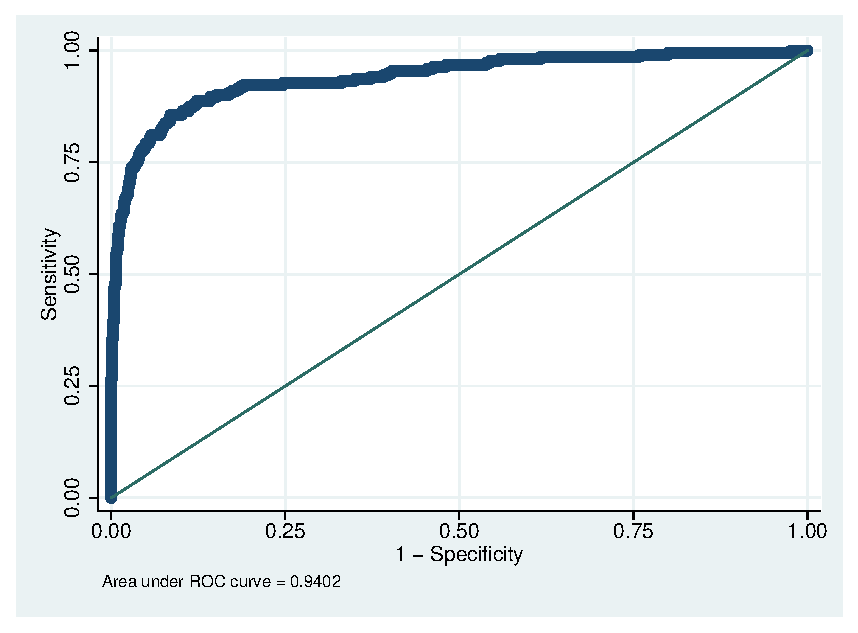
\includegraphics[height=3in]{Rysunki//PROC}
    \caption{\textbf{Krzywa ROC}}
\end{centering}
\end{figure}
\textit{\footnotesize{Źródło: Opracowanie własne.}} \\

\vspace{0.5cm}
\textbf{Tabela 45. Pole pod krzywą ROC }
\begin{stlog}
. lroc 
{\smallskip}
Probit model for oscar
{\smallskip}
number of observations =     1657
area under ROC curve   =   0.9402
 \end{stlog}
\textit{\footnotesize{Źródło: Opracowanie własne.}} \\

Pole pod krzywą ROC jest to procent dobrze zakwalifikowanych pozytywnych i negatywnych odpowiedzi przy różnych wyborach punktu rozdzielającego decyzję. Im bliższa jedynce wartość pola tym model jest lepiej dopasowany do danych wejściowych. Tabela 45 wskazuje na bardzo dobre dopasowanie modelu - pole pod krzywą ROC wynosi 0,9402.

\vspace{0.5cm}
\begin{figure}[h]
\begin{centering}
  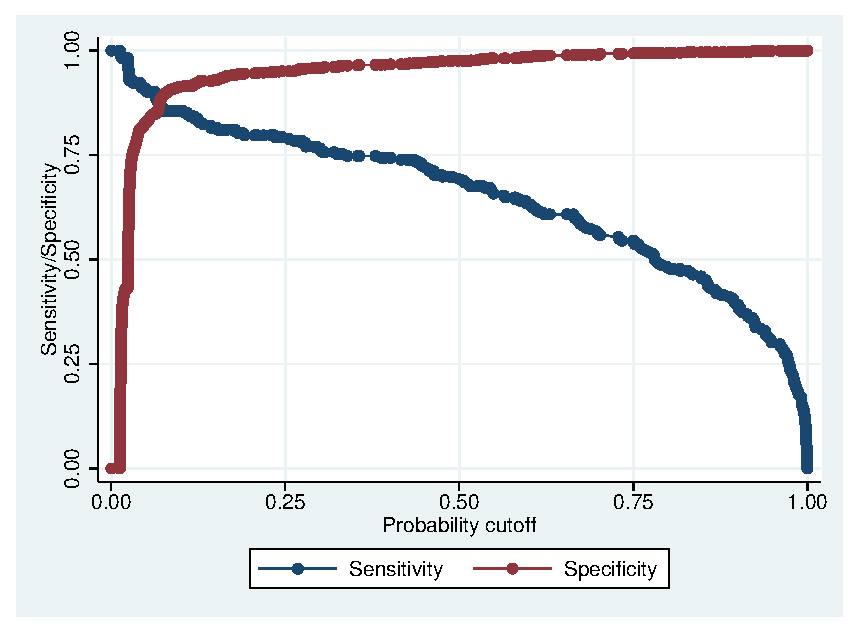
\includegraphics[height=3in]{Rysunki//SENS2}
    \caption{\textbf{Wrażliwość i Specyficzność}}
\end{centering}
\end{figure}
\textit{\footnotesize{Źródło: Opracowanie własne.}} \\

Wykres wrażliwości i specyficzności wskazuje prawdopodobieństwo ucięcia, czyli poziom rozgraniczenia maksymalizującego trafność klasyfikacji wartości dopasowanych. Z rysunku 8 wynika, iż najlepsze ucięcie powinno mieć miejsce w punkcie 0,05. Dla tego punktu wyznaczona została tablica klasyfikacji.

\vspace{0.5cm}
\textbf{Tabela 46. Tablica klasyfikacji dla punktu odcięcia 0,05}
\begin{stlog}
. lstat,cutoff(0.05)
{\smallskip}
Probit model for oscar
{\smallskip}
              \HLI{8} True \HLI{8}
Classified {\VBAR}         D            {\tytilde}D  {\VBAR}      Total
\HLI{11}{\PLUS}\HLI{26}{\PLUS}\HLI{11}
     +     {\VBAR}       202           249  {\VBAR}        451
     -     {\VBAR}        20          1186  {\VBAR}       1206
\HLI{11}{\PLUS}\HLI{26}{\PLUS}\HLI{11}
   Total   {\VBAR}       222          1435  {\VBAR}       1657
{\smallskip}
Classified + if predicted Pr(D) >= .05
True D defined as oscar != 0
\HLI{50}
Sensitivity                     Pr( +| D)   90.99\%
Specificity                     Pr( -|{\tytilde}D)   82.65\%
Positive predictive value       Pr( D| +)   44.79\%
Negative predictive value       Pr({\tytilde}D| -)   98.34\%
\HLI{50}
False + rate for true {\tytilde}D        Pr( +|{\tytilde}D)   17.35\%
False - rate for true D         Pr( -| D)    9.01\%
False + rate for classified +   Pr({\tytilde}D| +)   55.21\%
False - rate for classified -   Pr( D| -)    1.66\%
\HLI{50}
Correctly classified                        83.77\%
\HLI{50}
\end{stlog}
\textit{\footnotesize{Źródło: Opracowanie własne.}} \\
\vspace{1cm}

Tablica klasyfikacji dla punktu odcięcia równego 0,05 wskazuje, iż model poprawnie przewidział aż 202 spośród 222 filmów, które zdobyły Oscara, co oznacza, że wrażliwość modelu wyniosła 90,99\%. Specyficzność z kolei równa 82,65 wskazuje, iż model poprawnie zakwalifikował 1189 obserwacji spośród 1435 jako te, które statuetki nie uzyskały. Ogólny wskaźnik klasyfikacji modelu równy 83,77\%, wydaje się bardzo dobrym wynikiem. W związku z tym, iż współliniowość zmiennych objaśniających: _Igatunek_2, kraj_prod, przychody2000, ln_nom, ln_zg, ln_baf, milosc była już badana przy okazji modelu Logit nie ma potrzeby przeprowadzać testu na współliniowość ponownie. 

\phantomsection				% do hiperlinków dla sekcji w spisie treści
\section*{3.4 Wybór najlepszego modelu}
\addcontentsline{toc}{section}{3.4 Wybór najlepszego modelu}

W związku z tym, iż Liniowy Model Prawdopodobieństwa cechował się heteroskedastycznością reszt i wartościami dopasowanymi wykraczającymi poza przedział [0,1], wyboru modelu najlepiej reprezentującego dane należy dokonać pomiędzy modelem logitowym i probitowym. Dla obu tych modeli ich zagnieżdżone wersje nie miały prawidłowej formy funkcyjnej stąd też wybór będzie dokonywany pomiędzy dwoma modelami zawierającymi zlogarytmowane zmienne niezależne: ln_nom, ln_zg i ln_baf. 

\vspace{0.5cm}
\textbf{Tabela 47. Porównanie modeli Logit i Probit po transformacji}
\begin{stlog}
. fitstat, dif force
{\smallskip}
Measures of Fit for probit of oscar
{\smallskip}
Warning: Current model estimated by probit, but saved model estimated by logit
{\smallskip}
                               Current             Saved        Difference
Model:                          probit             logit
N:                                1657              1657                 0
Log-Lik Intercept Only        -652.655          -652.655             0.000
Log-Lik Full Model            -284.052          -286.079             2.027
D                              568.104(1649)     572.157(1649)       4.054(0)
LR                             737.207(6)        733.153(7)          4.054(1)
Prob > LR                        0.000             0.000             0.044
McFadden's R2                    0.565             0.562             0.003
McFadden's Adj R2                0.553             0.549             0.003
ML (Cox-Snell) R2                0.359             0.358             0.002
Cragg-Uhler(Nagelkerke) R2       0.659             0.656             0.003
McKelvey \& Zavoina's R2          0.602             0.610            -0.008
Efron's R2                       0.591             0.590             0.000
Tjur's Discrimination Coef       0.594             0.596            -0.002
Variance of y*                   2.511             8.425            -5.914
Variance of error                1.000             3.290            -2.290
Count R2                         0.937             0.937            -0.001
Adj Count R2                     0.527             0.532            -0.005
AIC                            584.104           588.157            -4.054
AIC/N                            0.353             0.355            -0.002
BIC                            619.993           631.460           -11.467
{\smallskip}
Difference of   11.467 in BIC provides very strong support for current model.
{\smallskip}
Note: p-value for difference in LR is only valid if models are nested.
\end{stlog}
\textit{\footnotesize{Źródło: Opracowanie własne.}} \\

Różnica pomiędzy modelami dla większości wskaźników determinacji jest niewielka, modele te są ze sobą silnie skorelowane (tabela 48). R$^2$ McFaddena, skorygowane R$^2$ McFaddena,  R$^2$ Efrona, kryteria informacyjne AIC i BIC oraz pole pod krzywą ROC (rysunek 7, tabela 49) wskazują, iż lepiej dopasowanym modelem jest model probitowy. Z kolei R$^2$ McKelvey'a \& Zavoina, skorygowane liczebnościowe R$^2$ oraz analiza literatury wskazują, iż do interpretacji oszacowań modelu należałoby użyć modelu logitowego. 

\vspace{2cm}
\textbf{Tabela 48. Współczynnik korelacji pomiędzy modelami Logit i Probit}
\begin{stlog}
. pwcorr prlogit prprobit 
{\smallskip}
             {\VBAR}  prlogit prprobit
\HLI{13}{\PLUS}\HLI{18}
     prlogit {\VBAR}   1.0000 
    prprobit {\VBAR}   0.9994   1.0000 
\end{stlog}
\textit{\footnotesize{Źródło: Opracowanie własne.}} \\

\vspace{0.5cm}
\begin{figure}[h]
\begin{centering}
  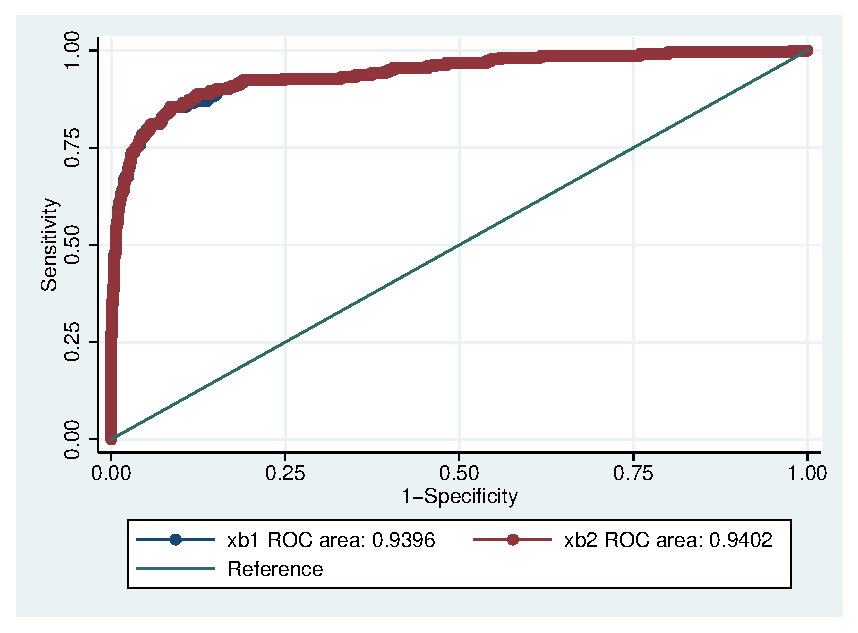
\includegraphics[height=3in]{Rysunki//PorownanieROC}
    \caption{\textbf{Krzywe ROC dla Logitu (niebieska linia) i Probitu (czerwona linia)}}
\end{centering}
\end{figure}
\textit{\footnotesize{Źródło: Opracowanie własne.}} \\

\vspace{0.3cm}
\textbf{Tabela 49. Porównanie krzywych ROC dla Logitu i Probitu}
\begin{stlog}
. roccomp oscar logit_fin probit_fin, graph summary
{\smallskip}
                              ROC                    {\DASH}Asymptotic Normal\HLI{2}
                   Obs       Area     Std. Err.      [95\% Conf. Interval]
\HLI{73}
logit_fin         1657     0.9396       0.0100        0.91998     0.95917
probit_fin        1657     0.9402       0.0100        0.92067     0.95975
\HLI{73}
Ho: area(logit_fin) = area(probit_fin)
    chi2(1) =     4.60       Prob>chi2 =   0.0319
\end{stlog}
\textit{\footnotesize{Źródło: Opracowanie własne.}} \\

W związku z wyraźnym wskazaniem bayesowskiego kryterium informacyjnego na model Probit (BIC mniejsze o 11,467) oraz z większością wskaźników determinacji bardziej korzystnych dla niego to właśnie ten model powinien być uznawany za najlepiej opisujący prawdopodobieństwo otrzymania nagrody Amerykańskiej Akademii Sztuki i Wiedzy Filmowej. 

W załączniku nr 1 do niniejszej pracy przedstawiona jest tabela zawierająca oszacowania parametrów i najważniejsze statystyki wszystkich modeli przedstawionych w tym rozdziale.